\graphicspath{{included-papers-tex/paper-6/}}

%\includedPaper{\textsc{paper vi - designer modeling through design style clustering}}{\textsc{paper vi - designer modeling through design style clustering}}{Alberto Alvarez, Jose Font, and Julian Togelius}

\includedPaper{\textsc{paper viii - Questgram [Qg]: Toward a Mixed-Initiative Quest Generation Tool}}{\textsc{paper viii - Questgram [Qg]: Toward a Mixed-Initiative Quest Generation Tool}}{Alberto Alvarez, Eric Grevillius, Elin Olsson, and Jose Font}

\normalfont
\textbf{\textsc{ABSTRACT}}

Quests are a core element in many games, especially \emph{role-playing} and \emph{adventure} games, where quests drive the gameplay and story, engage the player in the game’s narrative, and in most cases, act as a bridge between different game elements. The automatic generation of quests and objectives is an interesting challenge since this can extend the lifetime of games such as in \emph{Skyrim}, or can help create unique experiences such as in \emph{AI Dungeon}. This work presents Questgram [Qg], a mixed-initiative prototype tool for creating quests using grammars combined in a mixed-initiative level design tool. We evaluated our tool quantitatively by assessing the generated quests and qualitatively through a small user study. Human designers evaluated the system by creating quests \emph{manually}, \emph{automatically}, and through \emph{mixed-initiative}. Our results show the Questgram's potential, which creates diverse, valid, and interesting quests using quest patterns. Likewise, it helps engage designers in the quest design process, fosters their creativity by inspiring them, and enhance the level generation facet of the Evolutionary Dungeon Designer with steps towards intertwining both level and quest design.

\textbf{\textsc{PUBLISHED IN}}

The 16th International Conference on the Foundations of Digital Games (FDG), ACM, 2021.

\section*{Questgram [Qg]: Toward a Mixed-Initiative Quest Generation Tool}

\subsection{Introduction}

Defining quests and related concepts have been the focus of considerable research, where quests have been related to tasks, challenges, rewards, or as a storytelling device adding nuances to what a quest is~\citepeighth{p8Doran2011-questsMMORPGs,p8Breault2021-CONANQuestGen,p8Trenton2010-questpatterns,p8yu2020quest}. Most games have some quest driving the game's plot and gameplay. Adventure games, action-adventure games, and role-playing games (RPG) are among the main genres using quests~\citepeighth{p812-howard2008quests}, where most of these genres take place or containing some type of dungeon such as \emph{The Legend of Zelda}, \emph{Skyrim}, or \emph{The Binding of Isaac}. Dungeons as game content can be defined as a single level or set of levels containing enemies, treasures, hidden passages, puzzles, decorations, or Non-playable characters (NPC), thus creating space that allows the player to explore the unknown areas~\citepeighth{p8Dahlskog2015-patternsDungeonsGens}. Dungeons are a popular level design, especially within PCG~\citepeighth{p8shaker_procedural_2016,p8Yannakakis2018,p8Liapis2020-pcgWorkshop}, where it has been present ever since the 1970s in games such as \emph{Rogue}.

The increasing usage of Procedural Content Generation (PCG) in both research and industry~\citepeighth{p8Liapis2020-pcgWorkshop,p81-Lavender2016TheZD} has shown successful results regarding the efficiency of the game development process~\citepeighth{p8Pedersen2010-modelingPlayerExp} but also to generate a big amount of variation in games, increasing their replayability~\citepeighth{p8Smith2014-understandingPCG}. PCG can generate game content quickly such as missions and levels~\citepeighth{p8dormans2011generating}, content adapted to players~\citepeighth{p8hastings_evolving_2009}, or data-driven generation~\citepeighth{p8Green2018,p8summerville2018procedural}. Narrative and quest generation as objectives and goals has also been the focus of PCG~\citepeighth{p8Mason2019-LumeStoryGeneration,p8flodtol2020-WIPMakeSenseDungs,p8ammanabrolu2019-towardQuestGeneration}, where the aim has been to capture and use quest concepts and patterns to approach the generation, such as the work by Trenton et al.~\citepeighth{p8Trenton2010-questpatterns}, Kreminski and Wardrip-fruin~\citepeighth{p8Kreminski2018-SketchingStorylets}, Smith et al.~\citepeighth{p8Smith2011-situatingQuests} or Doran and Parberry~\citepeighth{p8Doran2011-questsMMORPGs}. 

Nevertheless, much of the content is still best made by humans, especially when subjective evaluations are needed~\citepeighth{p8shaker_procedural_2016}. To cope with this, one could use a mixed-initiative approach.
% Mixed-initiative focuses on the human-machine collaboration where both take part in the solution~\citepeighth{p8novick97-mixedInit}. 
Mixed-initiative Co-creativity (MI-CC) was introduced by Yannakakis et al., where both human and AI co-create and -design some game facet with a proactive initiative~\citepeighth{p8yannakakis2014micc}. MI-CC has been explored mainly for level design in tools such as the Sentient Sketchbook~\citepeighth{p8Liapis2013-sentientsketchbook}, Tanagra~\citepeighth{p8smith_tanagra:_2011}, Morai Maker~\citepeighth{p8guzdial-lvldsg-aiide-2018}, or the Evolutionary Dungeon Designer (EDD)~\citepeighth{p8Alvarez2020-ICMAPE}. EDD lets the user design interconnected room in a dungeon while receiving room suggestions adapted to their creation. Questgram is implemented in EDD, taking advantage of its level design capabilities and mixed-initiative approach.

% EDD is a mixed-initiative level design tool that lets the user design interconnected room in a dungeon while a MAP-Elites algorithm variant, IC MAP-Elites, generate and suggests adapted rooms. Questgram is implemented in EDD, taking advantage of its level design capabilities and mixed-initiative approach.

This research takes the quest analysis, quest patterns, and quest grammars identified by Doran and Parberry~\citepeighth{p8Doran2011-questsMMORPGs}, implements it in EDD, adapts it in a mixed-initiative approach for the creation of quest sequences, and extends it to work with level generation. The designer can create quests by adding manually available quest actions in a quest sequence and receive suggestions from the quest grammar that they might use to continue the quest, replace some part of the quest, or get inspiration to continue their quest. The available quest actions are related to the current dungeon layout. If modifying such dungeon renders invalid current quest parts, the designer is prompted to fix the quest manually or using actions suggested by the system. The system was evaluated quantitatively by assessing the diversity and incidence of quest actions, and qualitatively through a user study evaluating the experience, usability and suitability of the system.




% A world without a narrative to create meaning and make sense of the events that happen or a narrative without a world or space to take place creates a pointless system in most cases. This aligns with the view of Aarseth, who links the space to the quest in games being both level design and quests dependant on each other~\citepeighth{p8aarseth2005hunt}. A similar point is presented by Ashmore and Nitsche in relation to the games' interactivity as they discuss that a generated level without depth and context lacks interest for the final user~\citepeighth{p830-ashmore2007-questGeneratedWorld}. Conveniently, DEHn and lebowitz and kybartas and bidarra

% Narrative and quest generation has also been the focus of PCG, where it is in the most parts linked to the generation of levels

% Quests and it's definition has been the focus...
% Defining quests and related concepts have been the focus of multiple research, where quests have been related to tasks, challenges, rewards, or as a storytelling device adding nuances to what a quest is~\citepeighth{p8Doran2011-questsMMORPGs,31-breault2018let,Trenton2010-questpatterns,yu2020quest}. Most games have some type of quest driving the game's plot and gameplay. Adventure games, action-adventure games, and role-playing games (RPG) are among the main genres using quests~\citepeighth{p812-howard2008quests}, where most of these genres take place or containing some type of dungeon such as \emph{The Legend of Zelda}, \emph{Skyrim}, or \emph{The Binding of Isaac}. Dungeons as game content can be defined as a single level or set of levels that are set in an underground complex and is connected through an overworld with cities or a wilderness. Dungeons can contain enemies, treasures, hidden passages, puzzles, decorations, and Non-playable characters (NPC), thus creating space that allows the player to explore the unknown areas~\citepeighth{p8Dahlskog2015-patternsDungeonsGens}. Dungeons are a popular level design, especially within PCG~\citepeighth{p8shaker_procedural_2016,Yannakakis2018,Liapis2020-pcgWorkshop}, where it has been present in popular games ever since the 1970s with games such as \emph{Rogue}.


% Quests have been defined by Horward as "... a conceptual bridge that can help to join together many two-part or binary pairs [...] these include game and narrative, gaming and literature, technology and mythology and meaning and action~\citepeighth{p812-howard2008quests}”. Howard argues that quests unify both meaning and action, where meaning hails from strategic actions with thematic, narrative and personal implications, and actions being those that are meaningful for the player on the level of ideas, personal ambitions, benefits to society, and spiritual authenticity~\citepeighth{p812-howard2008quests}. Aarseth describes quests as concrete and attainable goals, and such can be hierarchic, concurrent, serial, or a combination of those. Further, Aarseth describes three basic quest types~\emph{Time-},~\emph{Place-}, and~\emph{Objective-oriented}, which can also be combined to form seven different quest types~\citepeighth{p8aarseth2005hunt}. 


% Similar definitions have been introduced relating quests to tasks, challenges, rewards, and as a storytelling mechanic have been introduced before, which adds more nuance~\citepeighth{p89-Doran2011-questsMMORPGs,31-breault2018let,Trenton2010-questpatterns,yu2020quest}, . 


% Similarly, Doran and Parberry~\citepeighth{p89-Doran2011-questsMMORPGs}, Trenton et al.~\citepeighth{p8Trenton2010-questpatterns}, Breault et al.~\citepeighth{p831-breault2018let} ~\citepeighth{p817-SoaresdeLima_HierarchicalgenQuests}


% Narrative and quest generation has been the focus of recent research in PCG, where the aim has been to capture quest concepts and quest patterns to approach quest generation such as the work by Trenton et al.~\citepeighth{p8Trenton2010-questpatterns}, Kreminski et al.~\citepeighth{p8Kreminski2018-SketchingStorylets} or Doran and Parberry~\citepeighth{p89-Doran2011-questsMMORPGs}. 


% On a bigger perspective, research on quest generation using PCG has been conducted by Parberry and Doran~\citepeighth{p89-Doran2011-questsMMORPGs}, Braualt et al~\citepeighth{p831-breault2018let}, and Dormans ~\citepeighth{p810-dormans2011generating}. This paper researches quest generation in a mixed-initiative procedural content generator.
%but none have been through mixed-initiative, thus making this research a starting point for a new research area to be explored within both PCG, mixed-initiative and narratives. 
% As one challenge of PCG in games is that it could ultimately lead to uninspiring and uncreative content~\citepeighth{p827-AraujoGameWorldsCreativity}, our research contributes to shifting from an automatic procedurally generated content to mixed authorship with the creative collaboration in focus.

% However, many parts are still best made by humans, especially when subjective evaluations are needed~\citepeighth{p84-shaker_procedural_2016}. To cope with this, one could use a mixed-initiative approach. Mixed-initiative focuses on the human-machine collaboration where both take part in the solution~\citepeighth{p85-novick97-mixedInit}. Mixed-initiative Co-creativity (MI-CC) was introduced by Yannakakis et al. where both human and AI co-create and -design some game facet with a proactive initiative~\citepeighth{p86-yannakakis2014micc}.


% EDD lets the user manually design interconnected rooms with a set of generic tiles and uses a MAP-Elites algorithm variant, IC MAP-Elites, to generate and suggest levels to the designer. Questgram is implemented in EDD making use of its level design capabilities and mixed-initiative approach.



% We implement our tool, the Questgram, in EDD, which lets the user manually design interconnected rooms with a set of generic tiles. EDD primary uses a variant of the MAP-Elites algorithm, IC MAP-Elites, to generate a vast amount of levels adapted to the designer's current design, evaluated by its composition, and several designer selected feature dimensions, and suggested to the designer to continue or replace their creation.

% forfor multiple genres for the creation of strategy games~\citepeighth{p8Liapis2013-sentientsketchbook}, the c

% MI-CC has been explored 

% Examples of previous game development tools using mixed-initiative co-creation (MI-CC) are Sentiment Sketchbook~\citepeighth{p85-novick97-mixedInit}, Tangara~\citepeighth{p87-smith_tanagra:_2011} and the evolutionary dungeon designer (EDD)~\citepeighth{p88-alvarez2019empowering}. EDD is a mixed-initiative dungeon designer for making dungeons for adventure games. The tool lets the user manually design rooms with enemies, treasures, chambers and an overall world structure that connects the different rooms. For the computing party of MI-CC, EDD uses evolutionary computations to procedurally generate content suggestions. The two parties collaborate and the evolutionary algorithms provide the user with alternatives, based on symmetry or similarity criteria. Currently, EDD does not have any narrative or story, which limits EDD’s potential, functionality and creative usage for the user. Narrative and quests are important to bring meaning into a game for the player as presented by Howard~\citepeighth{p812-howard2008quests}. 



% The increasing usage of Procedural Content Generation (PCG) in both research and industry~\citepeighth{p81-Lavender2016TheZD} has shown successful results regarding the efficiency of the game development process~\citepeighth{p82-Pedersen2010-modelingPlayerExp} but also to generate a big amount of variation in games, increasing their replayability. endless variations of a game, therefore making games “infinitely” replayable~\citepeighth{p83-Shaker2012EvolvingEvolution}. For example animation and the environment is taking a large part of a development budget~\citepeighth{p82-Pedersen2010-modelingPlayerExp}, which PCG can produce solutions efficiently. PCG can generate game content quickly, however some parts are still best made by humans~\citepeighth{p84-shaker_procedural_2016}. One solution is using a mixed-initiative approach. Which focuses on taking turns that are negotiated rather than determined by a single party regarding the modality of interaction~\citepeighth{p85-novick97-mixedInit}, in the case of game development, where the computer and human co-creates a solution to a problem. However, the two actors' contributions do not need to be the same~\citepeighth{p86-yannakakis2014micc}. 

% Examples of previous game development tools using mixed-initiative co-creation (MI-CC) are Sentiment Sketchbook~\citepeighth{p85-novick97-mixedInit}, Tangara~\citepeighth{p87-smith_tanagra:_2011} and the evolutionary dungeon designer (EDD)~\citepeighth{p88-alvarez2019empowering}. EDD is a mixed-initiative dungeon designer for making dungeons for adventure games. The tool lets the user manually design rooms with enemies, treasures, chambers and an overall world structure that connects the different rooms. For the computing party of MI-CC, EDD uses evolutionary computations to procedurally generate content suggestions. The two parties collaborate and the evolutionary algorithms provide the user with alternatives, based on symmetry or similarity criteria. Currently, EDD does not have any narrative or story, which limits EDD’s potential, functionality and creative usage for the user. Narrative and quests are important to bring meaning into a game for the player as presented by Howard~\citepeighth{p812-howard2008quests}. 

% On a bigger perspective, research on quest generation using PCG has been conducted by Parberry and Doran~\citepeighth{p89-Doran2011-questsMMORPGs}, Braualt et al~\citepeighth{p831-breault2018let}, and Dormans ~\citepeighth{p810-dormans2011generating}. This paper researches quest generation in a mixed-initiative procedural content generator.
% %but none have been through mixed-initiative, thus making this research a starting point for a new research area to be explored within both PCG, mixed-initiative and narratives. 
% As one challenge of PCG in games is that it could ultimately lead to uninspiring and uncreative content~\citepeighth{p827-AraujoGameWorldsCreativity}, our research contributes to shifting from an automatic procedurally generated content to mixed authorship with the creative collaboration in focus. 

% This links described by Howard

% The genres where quests appear are mainly adventure games, action-adventure games, and role-playing games (RPG)~\citepeighth{p812-howard2008quests}. Both RPGs and adventure games have a rich storyline, detailed characters, and involve exploration~\citepeighth{p813-aarseth2005hunt}. Dungeons as game content can be defined as a single level or set of levels that are set in an underground complex and is connected through an overworld with cities or a wilderness~\citepeighth{p814-Dahlskog2015-patternsDungeonsGens}. The cities can act as a replenishment zone where the player can do trades using found items or item upgrades. Dungeons can contain enemies, treasures, hidden passages, puzzles~\citepeighth{p814-Dahlskog2015-patternsDungeonsGens}, decorations, and Non-playable characters (NPC)~\citepeighth{p84-shaker_procedural_2016}, thus creating space that allows the player to explore the unknown areas~\citepeighth{p814-Dahlskog2015-patternsDungeonsGens}. Dungeons are a popular level design, especially within PCG~\citepeighth{p84-shaker_procedural_2016,13-aarseth2005hunt,15-Yannakakis2018}, where it has been present in popular games ever since the 1970s~\citepeighth{p816-Dahlskog2015-patternsDungeonsGens}. 

% Moreover, Aarseth defines quests as “a game that depends on mere movement from position A to position B"~\citepeighth{p813-aarseth2005hunt} and Howard defines it as “A quest is a middle term, a conceptual bridge that can help to join together many two-part or binary pairs [..] these include game and narrative, gaming and literature, technology and mythology and meaning and action”~\citepeighth{p812-howard2008quests}. This link between quest narrative, quests, and quest games has been proposed by Howard~\citepeighth{p812-howard2008quests}, arguing that quests unify both meaning and action. The meaning hails from strategic actions with thematic, narrative and personal implications, and actions being those that are meaningful for the player on the level of ideas, personal ambitions, benefits to society, and spiritual authenticity. Quests can be linked together like a chain to advance in the game’s story further~\citepeighth{p816-Dahlskog2015-patternsDungeonsGens} and give structure by limiting the player’s available choice through providing access to certain areas only in a specific order(s)~\citepeighth{p816-Dahlskog2015-patternsDungeonsGens}, thus making the game designer take control of the players’ agenda~\citepeighth{p813-aarseth2005hunt}. Besides being a fundamental element for narrative progression~\citepeighth{p817-SoaresdeLima_HierarchicalgenQuests}, quest affects the amount of space needed for a game’s landscape~\citepeighth{p810-dormans2011generating,13-aarseth2005hunt}. Aarseth describes three basic quest types~\emph{Time-},~\emph{Place-}, and~\emph{Objective-oriented}, which can also be combined to form seven different quest types.

% While many of the tools 

% This research takes the quest analysis, quest patterns, and quest grammars identified by Doran and Parberry~\citepeighth{p8Doran2011-questsMMORPGs}, implements it in EDD, adapts it in a mixed-initiative approach for the creation of quest sequences, and extends it to work with level generation. The designer is able to create quests by adding manually available quest actions in a quest sequence, and at the same time they get suggestions from the quest grammar that they might use to continue the quest, replace some part of the quest, or get inspiration to continue their quest. The available quest actions are related to the current dungeon layout. If modifying such dungeon renders invalid current quest parts, the designer is prompted to fix the quest, either manually or by using actions suggested by the system. Therefore, we also present a simple but clear step towards intertwining level design and narrative facets with the aim of holistic PCG~\citepeighth{p8Liapis2019-OrchestratingGames}. The system was evaluated through mixed-methods. First, it was evaluated quantitatively to assess the diversity and incidence of quest actions in multiple quest sequence generation in a sample dungeon. Second, a user study evaluated the usability, it was preliminary evaluated through a user study, where users used the tool in different modes and assessing its function, usability, and suitability.

% present a step towards holistic PCG~\citepeighth{p8Liapis2019-OrchestratingGames} by intertwining level design  and narrative 

% Our quest tool is implemented in EDD, a research framework for mixed-initiative content generation with a focus on level design.

%Discuss about the evaluation
%Introduce what the user can do, and how it is linked with the level part!


% implements it in 

% and extends it into a mixed-initiative approach

% This paper takes previous research by Parberry and Doran~\citepeighth{p89-Doran2011-questsMMORPGs} on classification of RPG quests, and uses it as the basis for integrating a mixed-initiative narrative generator on EDD. This approach does not only generate quests in a completely automatized fashion, as in~\citepeighth{p89-Doran2011-questsMMORPGs} and~\citepeighth{p831-breault2018let}, but lets users participate in the creative process by adding specific quest actions, such as “GOTO”, ”KILL”, “STEAL”~\citepeighth{p89-Doran2011-questsMMORPGs}, that can be extended upon user request with automatically generated actions. These procedurally generated actions use grammars to articulate the action generation with production rules, inspired by both Dorman’s~\citepeighth{p820-Dormans_AdventuresinLvlDes} work on action-adventure games and Parberry and Doran~\citepeighth{p89-Doran2011-questsMMORPGs}.  The generated quests will display the different series of quests available to the user in a list. The tool scans the room, thus eliminating quests that have a clear pre-condition, such as for the “KILL” action an enemy must have been placed. The user has the option to either use the generated actions, to manually place out different actions or use a combination of both to build up a full quest.

% PCG has several advantages such as  games can be produced faster and cheaper, thus making it possible for smaller teams without resources of large companies to create content rich games [27].
\subsection{Related Work}

Howard defined quests as "... a conceptual bridge that can help to join together many two-part or binary pairs [...] these include game and narrative, gaming and literature, technology and mythology and meaning and action~\citepeighth{p812-howard2008quests}". Howard argues that quests unify both meaning and action, where meaning hails from strategic actions with thematic, narrative, and personal implications; and actions being those that are meaningful for the player on the level of ideas, personal ambitions, benefits to society, and spiritual authenticity~\citepeighth{p812-howard2008quests}. Aarseth describes quests as concrete and attainable goals, and such can be hierarchic, concurrent, serial, or a combination of those. Further, Aarseth describes three basic quest types~\emph{Time-},~\emph{Place-}, and~\emph{Objective-oriented}, which can also be combined to form seven different quest types~\citepeighth{p8aarseth2005hunt}. Questgram is based on the quest analysis and proposed grammar by Doran and Parberry, constructed and extracted from analyzing over 750 quests from four RPGs and where they defined quests as a task given to the player that challenges them to complete some goals in exchange for some reward~\citepeighth{p8Doran2011-questsMMORPGs}. While helpful to understand quests as a whole, these definitions create a sense of ambiguity over different concepts surrounding quests. Yu et al.~\citepeighth{p8yu2020quest} proposed a generic quest definition in games that aims at unifying related concepts that appear in most of other's work, clearing ambiguity and easing it's use in PCG quest generation tools. Formally, they define a quest as $Q = \langle T, \leq, R \rangle$, where a quest $Q$ is a partially ordered set $\leq$ of tasks $T$ to be done to receive one or more rewards from a set $R$, which usually are in-game items.

% These definitions while helpful to understand quests as a whole; create a sense of ambiguity over different concepts surrounding quests. Yu et al.~\citepeighth{p8yu2020quest} propose a generic quest definition in games that aims at unifying related concepts that appear in most of other's work, clearing ambiguity and easing it's use in PCG quest generation tools. Formally, they define a quest as $Q = \langle T, \leq, R \rangle$, where a quest $Q$ is a partially ordered set $\leq$ of tasks $T$ to be done to receive one or more rewards from a set $R$, which usually is an in-game item. A task $t \in T$ is further defined as a 4-tuple $\langle C, M, I, R_{t} \rangle$, where $C$ is a precondition for the task, $M$ is the system for $C$ to be true, $I$ is the presentation of the quest, and $R_{t}$ is the set of rewards for completing task $t$.

\subsubsection{Story and Quest Generation}

Quests are fundamental elements in most games, driving the plot and player actions and providing goals and tasks to engage players with the game and the narrative. Doran and Parberry analyzed quests in four RPGs and found nine different "motivations" from NPC's, which resulted together with a specific strategy in a "verb-noun" pair, for example, "steal supplies" or "attack enemy". They used this grammar to generate quests while the user chose between nine identified NPC motivations~\citepeighth{p8Doran2011-questsMMORPGs}. Based on Doran and Parberry's action classification, Breault et al. developed an engine capable of creating quests similar to human-made ones, and since the engine generates quests based on the world state at the time of generation, the creation of possible quests increases as the game progresses~\citepeighth{p8Breault2021-CONANQuestGen}. 

One key characteristic in games is that they are interactive, and as such, can present choices to players. However, quests do not tend to provide such choice, especially in RPGs; rather, it is common that they are limited as a series of steps to follow.  An interesting approach is Questbrowser~\citepeighth{p8Sullivan2009-questbrowser}, a quest design brainstorming tool where the designer can query the system for ideas, alternatives, and possibilities on elements or concepts that foster designers' creativity and help make quests playable (i.e., adding choice for players). However, presenting choices to players could create competing objectives for designers as they want to impose their narrative but, at the same time, want to create adaptable experiences for players. %Aarseth~\citepeighth{p8Aarseth2012-Narrativetheory} discusses and analyzes this from the perspective of kernels, events that makes a story recognizable, and satellites, dispensable events that could be removed or changed. One example is Fa\c{c}ade~\citepeighth{p8mateas2003-faccade}, where players' actions are fundamental as transition points that are taken in consideration when planning and adding subsequent beats that can change the kernel events of the game; adapting the story to the player.

Planning algorithms are a common technique to compose stories and quests meaningfully and with some partial-ordering~\citepeighth{p8young2013-plansNarrGen,p8Porteous2017-PlanningTechnologiesIS}, focusing and optimizing character believability together with multi-agent systems~\citepeighth{p8Riedl2005-charBelievMulti,p8Riedl2006-StoryPlanningCreativity}, replicating common quests and quest patterns~\citepeighth{p8Doran2011-questsMMORPGs,p8Trenton2010-questpatterns,p831-breault2018let}, or identifying fundamental units and assembling them based on various pre-conditions~\citepeighth{p8Kreminski2018-SketchingStorylets,p8Garbe2019-StoryletsAssembler}. Kreminski and Wardrip-Fruin~\citepeighth{p8Kreminski2018-SketchingStorylets} mapped and compared multiple storylets-based systems and proposed the use of storylets, which are discrete, atomic, and recombinable narrative chunks, to assemble narratives based on a set of preconditions to create different narrative structures. Storylets were used by Garbe et al. in the StoryAssembler to generate dynamic narratives, which attempts to create a valid story with a planner using a set of provided storylets and storytelling goals that the planner uses as objective~\citepeighth{p8Garbe2019-StoryletsAssembler}. 

% Planning algorithms 

% representative events of a story, and satellites, dispensable 

% Interactive Storytelling 

% While presenting choices to players is beneficial,

% Presenting choices to players


% An interesting approach is Questbrowser~\citepeighth{p8Sullivan2009-questbrowser}, a quest design brainstorming tool using the common-sense database ConceptNet. In Questbrowser, the designer can query the system for ideas, alternatives, and possibilities on elements or concepts, that then can foster the creativity of designers and help make quests playable (i.e., adding choice for players). While presenting choices to players is beneficial, Presenting choices to players

% The discussion on presenting choices to players roots in the 

% Sullivan et al.~\citepeighth{p8Sullivan2009-questbrowser} analyzed and explored this situation with Questbrowser, a quest design brainstorming tool using the common-sense database ConceptNet, that allows and helps designers create meaningful quest design and choices for players. In Questbrowser, the designer can query the system for ideas, alternatives, and possibilities on elements or concepts, that then can foster the creativity of designers and help make quests playable (i.e., adding choice for players).

% challenges for   Questbrowser uses   and explored an approach, Questbrowser, to make quests playable (i.e., adding choice for players). Questbrowser is a quest design brainstorming tool that allows  Questbrowser uses 


% Sullivan et al.~\citepeighth{p8Sullivan2009-questbrowser} analyzed this situation and explored an approach, Questbrowser, to make quests playable (i.e., adding choice for players). Questbrowser is a quest design brainstorming tool that allows  Questbrowser uses 

% Through Questbrowser 

% Questbrowser  explores this with



% Kreminski and Wardrip-Fruin~\citepeighth{p8Kreminski2018-SketchingStorylets} mapped and compared multiple storylets-based systems and proposed the use of storylets to assemble narratives based on a set of preconditions with the goal of creating different narrative structures. Storylets are discrete, atomic, and recombinable narrative chunks, tested by Kreminski et al. with \emph{Felt} a story sifter that used parametrized storylets to produce story arcs~\citepeighth{p8Kreminski2019-FeltStorySifter}, and as a core component in the StoryAssembler . 

% Furthermore, Kreminski and Wardrip-Fruin~\citepeighth{p8Kreminski2018-SketchingStorylets} mapped and compared multiple storylets-based systems and proposed the use of storylets, which are discrete, atomic, and recombinable narrative chunks, to assemble narratives based on a set of preconditions with the goal of creating different narrative structures. While not explicitly quest generation, Kreminski et al. introduced \emph{Felt} a story sifter that used parametrized storylets to produce story arcs


% Moreover, since Questgram functions alongside a level generator, it is critical to discuss work that attempts to generate both facets and why this is important.
Moreover, Questgram functions within EDD's level design tool, which means both would function in relation to each other. Kybartas and Bidarra discussed the relation between plot and space, focusing on the degree of automation for story elements. This resulted in six categories: \emph{automated space}, \emph{constrained space}, \emph{space simulation}, \emph{space modification}, and \emph{manual space that builds a gradient between automatic and manual generation}~\citepeighth{p8kybartas2016survey}. Ashmore and Nitsche investigated a player-centric quest generation, where the progression through level generation is achieved with a "key and lock" structure, which results in a bridge between the generated space and the quests~\citepeighth{p8ashmore2007-questGeneratedWorld}.

% . The player engages in the quests to find the "key" to overcome the obstacle, thus blocking the player's progress in a flexible way, which according to Ashmore and Nitsche

% They argue that even with breaking down the narrative in sub-components, the goal of an automatic narrative creation tool there would still be a large presence of a human author, as so, benefitting mixed-initiative methods but opening up new research questions for fully automatic methods~\citepeighth{p8kybartas2016survey}.

Dormans and Bakkes used two grammars to generate both missions and game space, where the latter was informed by the first. Missions are generated using graph grammars, creating a non-linear structure suited for exploration, while extended shape grammar generates the corresponding space required~\citepeighth{p8dormans2011generating}. Further, Flodhag et al. use the information from levels co-created in \emph{EDD} and categorize them based on the meso-patterns within them to present a set of main and side objectives to designers in their dungeon~\citepeighth{p8flodtol2020-WIPMakeSenseDungs}. Hartsook et al. explore the creation of complete RPGs from a story created by either a computational system or human-authored and a set of player preferences. Their approach creates and represents game worlds as transition graphs based on a story composed of plot points, player's playstyle preferences, and designer constraints~\citepeighth{p8hartsook2011-storyWorlds}. 

% Similar to Dormans and Bakes approach, Abuzuraiq et al. presented taksim that uses constrained graph partitioning


% ADDITION TO DORMANS - Van der Linden et at. have proposed using gameplay grammar-based levels to generate dungeon levels, being able to significantly improve the design of procedurally generated levels [21].


% which is critical given that Questgram functions alongside a level generator.


% Add references to other approaches such as taksim~\citepeighth{p8abuzuraiq2019-taksim}, research from Mark Riedl~\citepeighth{p8Tambwekar2019-ControllableNeuralPlot}. Storylets~\citepeighth{p8Kreminski2018-SketchingStorylets,Garbe2019-StoryletsAssembler}, etc. There was another good one from the PCG workshop 2018 (gotcha)~\citepeighth{p8Smith2018-GraphBasedGeneration}.

% There are a variety of methods for procedurally creating content such as constructive methods, producing only one output per run, or search-based methods, which use evolutionary algorithms to search for good content according to Darwinian evolution principles. One constructive approach is using grammars [4], for example, Dorman’s [20] conducted research on using two-layered grammars to generate both gameplay and game space [4]. Dividing missions and spaces as separate structures and generating the content in two individual steps [20]. Missions are generated using graph grammars, creating a non-linear structure suited for exploration while extended shape grammar generates the corresponding space required [20]. Van der Linden et at. have proposed using gameplay grammar-based levels to generate dungeon levels, being able to significantly improve the design of procedurally generated levels [21].

 
% Doran and Parberry use a grammar constructed and extracted from analysing over 750 quests from four RPGs, to generate quests while the user simply chose between nine identified NPC motivations. Their work, defined quests as a task given to the player that challenges them to complete some goals in exchange of some reward~\citepeighth{p89-Doran2011-questsMMORPGs}. 

% Questgram is based on the quest analysis and proposed grammar by Doran and Parberry~\citepeighth{p89-Doran2011-questsMMORPGs}, where they found nine different "motivations" from NPC´s which resulted together with a specific strategy in a “verb-noun” pair, for example, “steal supplies”. This derived into twenty atomic actions.

% Doran and Parberry use a grammar constructed and extracted from analysing over 750 quests from four RPGs, to generate quests while the user simply chose between nine identified NPC motivations. Their work, defined quests as a task given to the player that challenges them to complete some goals in exchange of some reward~\citepeighth{p89-Doran2011-questsMMORPGs}.  

% Quest generation 
% Quest generation has been approached in multiple ways, although focusing on one way or another in quest patterns.  

% Quest generation has been approach in multiple ways 


% Quest generation provides unique opportunities to games such as increasing replayability, 

% As most games have some type of quest driving the plot and the player actions, and providing goals and tasks to motivate players; is normal that quest generation has been focused by the AI community. Quest generation provides unique opportunities to games such as increasing replayability

% Quests are core elements to drive the plot of game
% Quests are core elements in most games, where they are used as a means to drive the plot, the actions 
% Narrative is a fundamental element in games, which as it helps creating immersion 

% Given that most games have some type of quest driving the plot and the player actions, and providing goals and tasks to motivate players; quest generation has gained interest from the AI community. 

% Level and narrative have been 
% which is critical given that Questgram functions alongside a level generator.

% For quest generation Parberry and Doran has categorized quests based on NPC’s motivations with the goal of autonomous generation [9]. Other research  within autonomous generation is Ashmore and Nitsche [30], investigating a player centric quest generation, where the progression through level generation is achieved with “key and lock” structure.


% Games where the world is procedurally generated, encourage exploration, while games, where levels are procedurally generated, encourages replayability [15]. There is different type of replayability as Smith presents [28], reacting in a surprising environment (the game plays different content at each attempt), building generator strategies (experiencing different content and having the opportunity to build strategies around the content generator) and practicing in different environment (the game lets the player experience new challenges but of the same kind) [28]~\citepeighth{p828-UnderstandingPCG}.


\subsubsection{Mixed-Initiative Co-Creativity}

% \textbf{Present EDD~\citepeighth{p8alvarez2019empowering,Alvarez2020-ICMAPE}, Geminate~\citepeighth{p8kreminski2020-Germinate}, the work I am just reading from Kreminski as well.}

MI-CC is a paradigm where both humans and AI have a proactive initiative in the collaboration to co-create some creative content~\citepeighth{p8yannakakis2014micc,p8liapis2016mixed}. Both human and AI leverage on each other's strengths to achieve the task and continuously negotiate to determine roles; thus, collaborating as a team~\citepeighth{p8Allen99-MIinteraction}. One critical aspect of MI-CC systems is the link between these systems and theories of computational and human creativity, where a main focus of MI-CC is on fostering human's creativity while reducing their workload~\citepeighth{p8Liapis2016-CanComputersFosterCreativity,p8Alvarez2018}.

The \emph{Sentient Sketchbook} is an MI-CC tool for the co-creation of strategy games where the designer focused on creating low-resolution sketches, and the computational designer suggested variations generated with different evolutionary algorithms~\citepeighth{p8Liapis2013-sentientsketchbook}. Cicero is an MI-CC system that helps designers create complete games using a recommender system and A-Priori to suggest what content might be added next regarding sprites, mechanics, rules, or interactions~\citepeighth{p8machado2019pitako}. Another interesting MI-CC system is \emph{Why Are We Like This? (WAWLT)} where two players can develop a story transcript while supported by an AI system with tools to inspect the story world and with suggestions to direct the plot~\citepeighth{p8Kreminski2020-WAWLT}.

% \emph{Germinate} is an MI-CC system to co-create rhetorical games that allow designers to focus on a higher level, specifying constraints and properties of games they want the generator to create, and iteratively changing these based on the generator's output~\citepeighth{p8kreminski2020-Germinate}. 

EDD is an MI-CC system where the designer can create interconnected rooms that compose a dungeon while receiving a set of diverse suggestions using the IC MAP-Elites evolutionary algorithm driven by level design patterns and considering the designer's current design. The designer can interact with the suggestion system by locking tiles, editing their design, and selecting and interacting with hyper-parameters of IC MAP-Elites~\citepeighth{p8Alvarez2018a,p8Alvarez2020-ICMAPE}


% The designer can interact with the suggestion system by locking tiles (explicitly indicating what they want to preserve)~\citepeighth{p8Alvarez2018a}, by their design, by choosing suggestions which train a preference model~\citepeighth{p8Alvarez2020-DesignerPreference}, and by selecting multiple hyper-parameters of the evolutionary approach~\citepeighth{p8Alvarez2020-ICMAPE}. 

% Recently, an automatic dungeon assessment was introduced in EDD, which present a set of objectives to the designer based on what they created~\citepeighth{p8flodtol2020-WIPMakeSenseDungs}. Questgram builds on top of EDD and takes advantage of it's mixed-initiative perspective, the levels that are created, and the objectives that are identified. 


% Questgram is a prototype tool aiming at creating an MI-CC quest generation system that builds on top of EDD an MI-CC system for creating dungeon levels.

% an automatic dungeon evaluation was introduced in EDD that assess the dungeon and the different patterns that 


% However, while helpful to understand quests as a whole, quests and its components have been defined multiple times in research creating a sense of ambiguity over different concepts surrounding quests as discussed by Yu et al.~\citepeighth{p8yu2020quest}. Yu et al.~\citepeighth{p8yu2020quest} propose a generic quest definition in games that aims at unifying related concepts that appear in most of other's work, clearing ambiguity and easing it's use in PCG quest generation tools. Formally, they define a quest as $Q = \langle T, \leq, R \rangle$, where a quest $Q$ is a partially ordered set $\leq$ of tasks $T$ to be done to receive one or more rewards from a set $R$, which usually is an in-game item. A task $t \in T$ is further defined as a 4-tuple $\langle C, M, I, R_{t} \rangle$, where $C$ is a precondition for the task, $M$ is the system for $C$ to be true, $I$ is the presentation of the quest, and $R_{t}$ is the set of rewards for completing task $t$.

% Furthermore, Questgram is based on the quest analysis and proposed grammar by Doran and Parberry, where they found nine different "motivations" from NPC´s which resulted together with a specific strategy in a “verb-noun” pair, for example, “steal supplies”. This derived into twenty atomic actions~\citepeighth{p89-Doran2011-questsMMORPGs}. In their work, they use the grammar to generate quests while the user simply chose between the different motivations. Their work, defined quests as a task given to the player that challenges them to complete some goals in exchange of some reward.  

% Parberry and Doran found 9 different “motivations” from NPC´s which resulted together with a specific strategy in a “verb-noun” pair, for example, “steal supplies”. This derived into twenty atomic actions~\citepeighth{p89-Doran2011-questsMMORPGs}. A quest can be broken down into several side-quests [9], and be optional and unrelated to the main story-line~\citepeighth{p815-Yannakakis2018,18-fundamentalsGameDesign}.

% Yu et al.~\citepeighth{p8yu2020quest} propose a quest definition that aims at unifying related concepts that appear in most of other's work, and formalizing it  specifically defining quests as a partially ordered set of tasks that must be completed to receive one or more rewards. Formally, they define quest as $Q = \langle T, \leq, R \rangle$, 


% which is a partially ordered set $\leq$ of tasks $T$ that must be completed to receive a reward $R$, Reward is defined as $r \in R$, and Task as


% Formally, they define quests as a partially ordered set of tasks that must be completed to receive a reward $Q = \langle T, \leq, R \rangle$, Reward as 

% Yu et al.~\citepeighth{p8yu2020quest} propose a generic quest definition that aims at unifying related concepts that appear in most of other's work, specifically a quest is defined as a partially ordered set of tasks to be done to receive one or more rewards from a set of

% Yu et al.~\citepeighth{p8yu2020quest} propose a generic quest definition in games that aims at unifying related concepts that appear in most of other's work, clearing ambiguity and easing it's use in PCG quest generation tools. Formally, they define a quest as $Q = \langle T, \leq, R \rangle$, where a quest $Q$ is a partially ordered set $\leq$ of tasks $T$ to be done to receive one or more rewards from a set $R$, which usually is an in-game item. A task $t \in T$ is further defined as a 4-tuple $\langle C, M, I, R_{t} \rangle$, where $C$ is a precondition for the task, $M$ is the system for $C$ to be true, $I$ is the presentation of the quest, and $R_{t}$ is the set of rewards for completing task $t$.

% A reward $r \in R$ 

% formalizing this to ease it's use in PCG quest generation tools. Formally, they define a quest as $Q = \langle T, \leq, R \rangle$, which 

%%%%%%%%%%%%%%%%%%%%%%% THIS HAS NOT BEEN DONE! %%%%%%%%%%%%%%%%%%%%%
%%%%%%%%%%%%%%%%%%%%%%% THIS HAS NOT BEEN DONE! %%%%%%%%%%%%%%%%%%%%%
%%%%%%%%%%%%%%%%%%%%%%% THIS HAS NOT BEEN DONE! %%%%%%%%%%%%%%%%%%%%%

% \subsubsection{Adventure Games, Dungeons, and Quests}

% \textbf{Here we want to write about quests and dungeon games}

% The genres where quests appear are mainly adventure games, action-adventure games, and role-playing games (RPG)~\citepeighth{p812-howard2008quests}. Both RPGs and adventure games have a rich storyline, detailed characters, and involve exploration~\citepeighth{p8aarseth2005hunt}. Dungeons as game content can be defined as a single level or set of levels that are set in an underground complex and is connected through an overworld with cities or a wilderness~\citepeighth{p8Dahlskog2015-patternsDungeonsGens}. The cities can act as a replenishment zone where the player can do trades using found items or item upgrades. Dungeons can contain enemies, treasures, hidden passages, puzzles~\citepeighth{p8Dahlskog2015-patternsDungeonsGens}, decorations, and Non-playable characters (NPC)~\citepeighth{p8shaker_procedural_2016}, thus creating space that allows the player to explore the unknown areas~\citepeighth{p8Dahlskog2015-patternsDungeonsGens}. Dungeons are a popular level design, especially within PCG~\citepeighth{p8shaker_procedural_2016,aarseth2005hunt,Yannakakis2018}, where it has been present in popular games ever since the 1970s~\citepeighth{p8Dahlskog2015-patternsDungeonsGens}. 

% Moreover, Aarseth defines quests as “a game that depends on mere movement from position A to position B"~\citepeighth{p8aarseth2005hunt} and Howard defines it as “A quest is a middle term, a conceptual bridge that can help to join together many two-part or binary pairs [..] these include game and narrative, gaming and literature, technology and mythology and meaning and action”~\citepeighth{p812-howard2008quests}. This link between quest narrative, quests, and quest games has been proposed by Howard~\citepeighth{p812-howard2008quests}, arguing that quests unify both meaning and action. The meaning hails from strategic actions with thematic, narrative and personal implications, and actions being those that are meaningful for the player on the level of ideas, personal ambitions, benefits to society, and spiritual authenticity. Quests can be linked together like a chain to advance in the game’s story further~\citepeighth{p8Dahlskog2015-patternsDungeonsGens} and give structure by limiting the player’s available choice through providing access to certain areas only in a specific order(s)~\citepeighth{p8Dahlskog2015-patternsDungeonsGens}, thus making the game designer take control of the players’ agenda~\citepeighth{p8aarseth2005hunt}. Besides being a fundamental element for narrative progression~\citepeighth{p817-SoaresdeLima_HierarchicalgenQuests}, quest affects the amount of space needed for a game’s landscape~\citepeighth{p8dormans2011generating,aarseth2005hunt}. Aarseth describes three basic quest types~\emph{Time-},~\emph{Place-}, and~\emph{Objective-oriented}, which can also be combined to form seven different quest types.

% Furthermore, Parberry and Doran found 9 different “motivations” from NPC´s which resulted together with a specific strategy in a “verb-noun” pair, for example, “steal supplies”. This derived into twenty atomic actions~\citepeighth{p89-Doran2011-questsMMORPGs}. A quest can be broken down into several side-quests [9], and be optional and unrelated to the main story-line~\citepeighth{p8Yannakakis2018,18-fundamentalsGameDesign}.

% \subsubsection{Narrative and Quest Generation}

%%%%%%%%%%%%%%%%%%%%%%% THIS HAS NOT BEEN DONE! %%%%%%%%%%%%%%%%%%%%%
%%%%%%%%%%%%%%%%%%%%%%% THIS HAS NOT BEEN DONE! %%%%%%%%%%%%%%%%%%%%%
%%%%%%%%%%%%%%%%%%%%%%% THIS HAS NOT BEEN DONE! %%%%%%%%%%%%%%%%%%%%%

% Examples of games with procedurally generated content and dungeons are The Elder Scrolls V: Skyrim, Diablo, and Rogue  [4]. Skyrim uses PCG to create missions and adventures [27],  Diablo to create maps and the type, number, and placements of items and monsters[15]. Rogue is a classic example of early use of PCG with dungeons and even spawning a genre called Roguelikes [4]. These successful games and the unique challenges in their design have made dungeons an active and attractive PCG subject [4]. It  can also  increase replayability and become a design tool to assist designers, such as mixed-initiative systems [4]. The usage of PCG has been investigated by Aruajo and Souto through a case study of No Man’s Sky and state of the art study [27]. Aruajo and Souto  have proposed three recommendations for PCG in games with the desired effect. 

% \begin{itemize}
%     \item Basic - When PCG  is used to generate content, thus making developers able to work on predetermined templates instead of creating from scratch. Aruajo and Souto argue smaller studios with no or little PCG usage should focus on shorter games with interesting core design.
%     \item Intense - When PCG is used to increase game time and enjoyment but does not detract from possibilities provided by the game. 
%     \item Core - When PCG is used as a core element of the game. This requires a larger fine turning to make sure the players interest in the game is kept over the curse of the gameplay.
% \end{itemize}

% While PCG can offer a great quantity content wise, it could ultimately turn into uncreative and uninteresting content. The challenge when creating an interesting world is to balance between the need for a long game and to fill it with interesting stories and elements, thus arguing for a  content quality over a content quantity approach [27].

%%%%%%%%%%%%%%%%%%%%%%% THIS HAS NOT BEEN DONE! %%%%%%%%%%%%%%%%%%%%%
%%%%%%%%%%%%%%%%%%%%%%% THIS HAS NOT BEEN DONE! %%%%%%%%%%%%%%%%%%%%%
%%%%%%%%%%%%%%%%%%%%%%% THIS HAS NOT BEEN DONE! %%%%%%%%%%%%%%%%%%%%%

% Games where the world is procedurally generated, encourage exploration, while games, where levels are procedurally generated, encourages replayability [15]. There is different type of replayability as Smith presents [28], reacting in a surprising environment (the game plays different content at each attempt), building generator strategies (experiencing different content and having the opportunity to build strategies around the content generator) and practicing in different environment (the game lets the player experience new challenges but of the same kind) [28].

% Definitely point towards Yu et al. quest definition and breakdown~\citepeighth{p8yu2020quest}

% Add references to other approaches such as taksim~\citepeighth{p8abuzuraiq2019-taksim}, research from Mark Riedl~\citepeighth{p8Tambwekar2019-ControllableNeuralPlot}. Storylets~\citepeighth{p8Kreminski2018-SketchingStorylets,Garbe2019-StoryletsAssembler}, etc. There was another good one from the PCG workshop 2018 (gotcha)~\citepeighth{p8Smith2018-GraphBasedGeneration}.

% There are a variety of methods for procedurally creating content such as constructive methods, producing only one output per run, or search-based methods, which use evolutionary algorithms to search for good content according to Darwinian evolution principles. One constructive approach is using grammars [4], for example, Dorman’s [20] conducted research on using two-layered grammars to generate both gameplay and game space [4]. Dividing missions and spaces as separate structures and generating the content in two individual steps [20]. Missions are generated using graph grammars, creating a non-linear structure suited for exploration while extended shape grammar generates the corresponding space required [20]. Van der Linden et at. have proposed using gameplay grammar-based levels to generate dungeon levels, being able to significantly improve the design of procedurally generated levels [21].

% The relation between plot and space have been further presented by Kybartas and Bidarra, with focus on the degree of automation for story elements. This resulted in five categories: automated space, constrained space, space simulation, space modification,  manual space that builds a gradient between automatic and manual generation~\citepeighth{p8kybartas2016survey}. Kybartas and Bidarra argue that even with breaking down narrative in sub-components, the goal of an automatic narrative creation tool there would still be a large presence of a human author, as so, benefitting mixed initiative methods but opening up new research questions for fully automatic methods~\citepeighth{p8kybartas2016survey}.

% For quest generation Parberry and Doran has categorized quests based on NPC’s motivations with the goal of autonomous generation [9]. Other research  within autonomous generation is Ashmore and Nitsche [30], investigating a player centric quest generation, where the progression through level generation is achieved with “key and lock” structure.

% More quest generation research has been conducted by Breault et al. following Parberry and Dorans action classification. The findings were that their developed engine was capable of creating quests similar to human written ones, and because the engine generates quests based on the world state at the time of generation, the creation of possible quests increases as the game progresses [31]. 

%%%%%%%%%%%%%%%%%%%%%%% THIS HAS NOT BEEN DONE! %%%%%%%%%%%%%%%%%%%%%
%%%%%%%%%%%%%%%%%%%%%%% THIS HAS NOT BEEN DONE! %%%%%%%%%%%%%%%%%%%%%
%%%%%%%%%%%%%%%%%%%%%%% THIS HAS NOT BEEN DONE! %%%%%%%%%%%%%%%%%%%%%
\subsection{Quest Generation}

\begin{figure*}[t]
    \centering
    \captionsetup[subfigure]{width=0.9\textwidth}
    \begin{subfigure}[t]{1\textwidth}
        \centering
        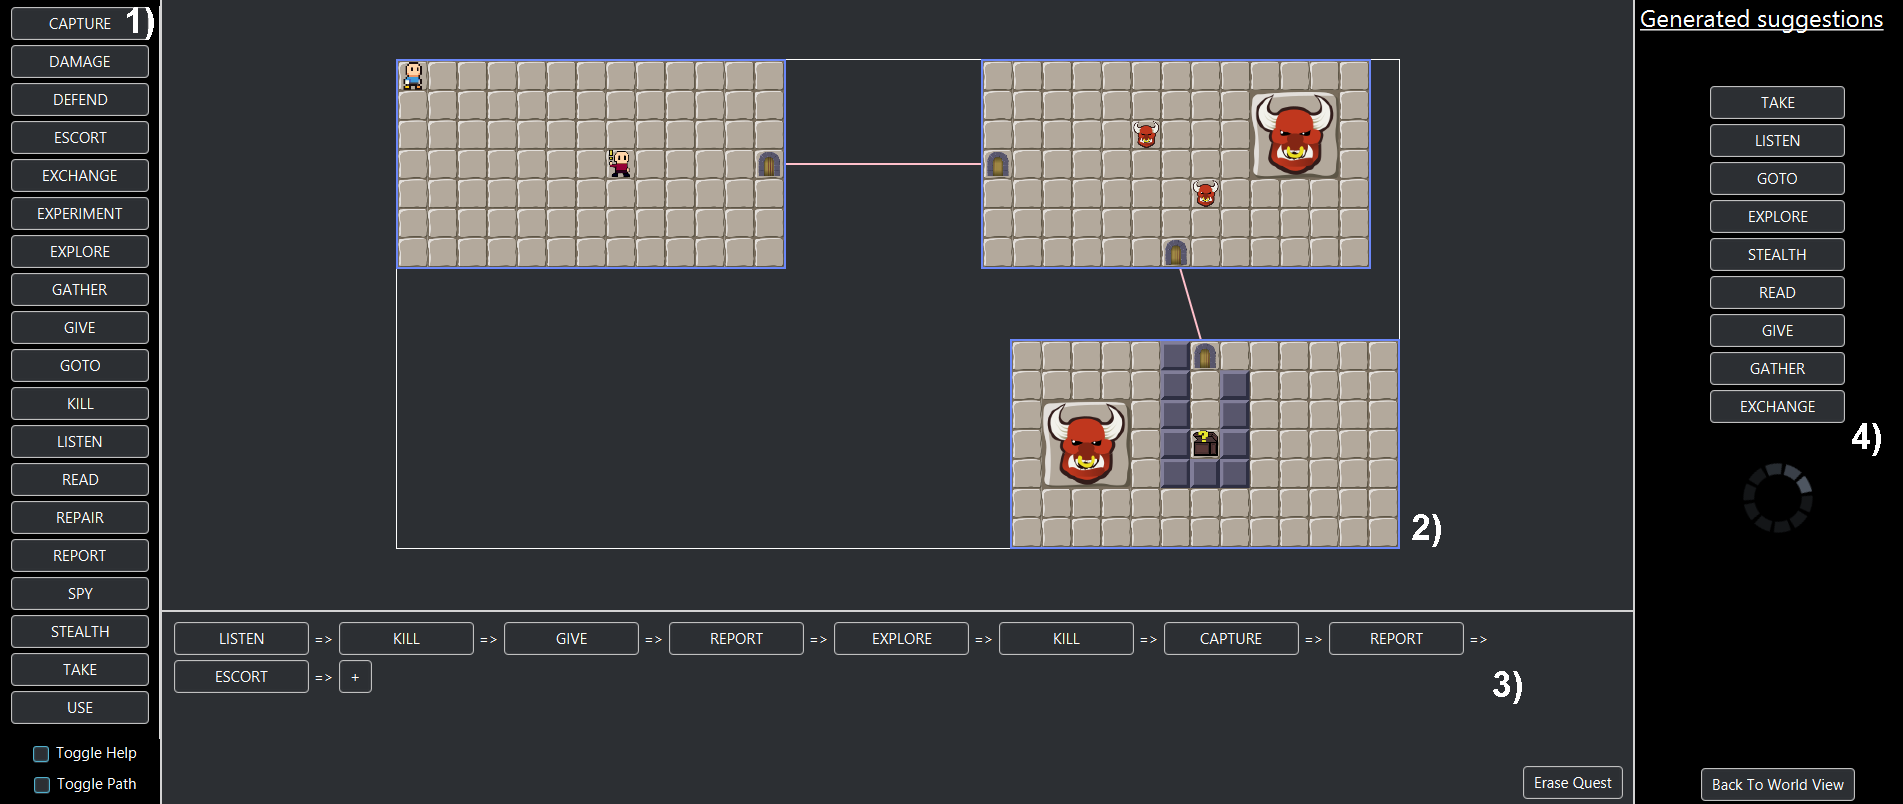
\includegraphics[width=.9\textwidth]{included-papers-tex/paper-8/figures/main.png}
        \caption{Overview of the GUI used for the design of quests in EDD. 1) The possible quest actions, 2) the dungeon created thus far by the designer, 3) the quest sequence, and 4) the suggestions from the grammar.}
        \label{figs:GUI:overview}
    \end{subfigure} \hfill% \
     
    \begin{subfigure}[t]{0.48\textwidth}
        \centering
         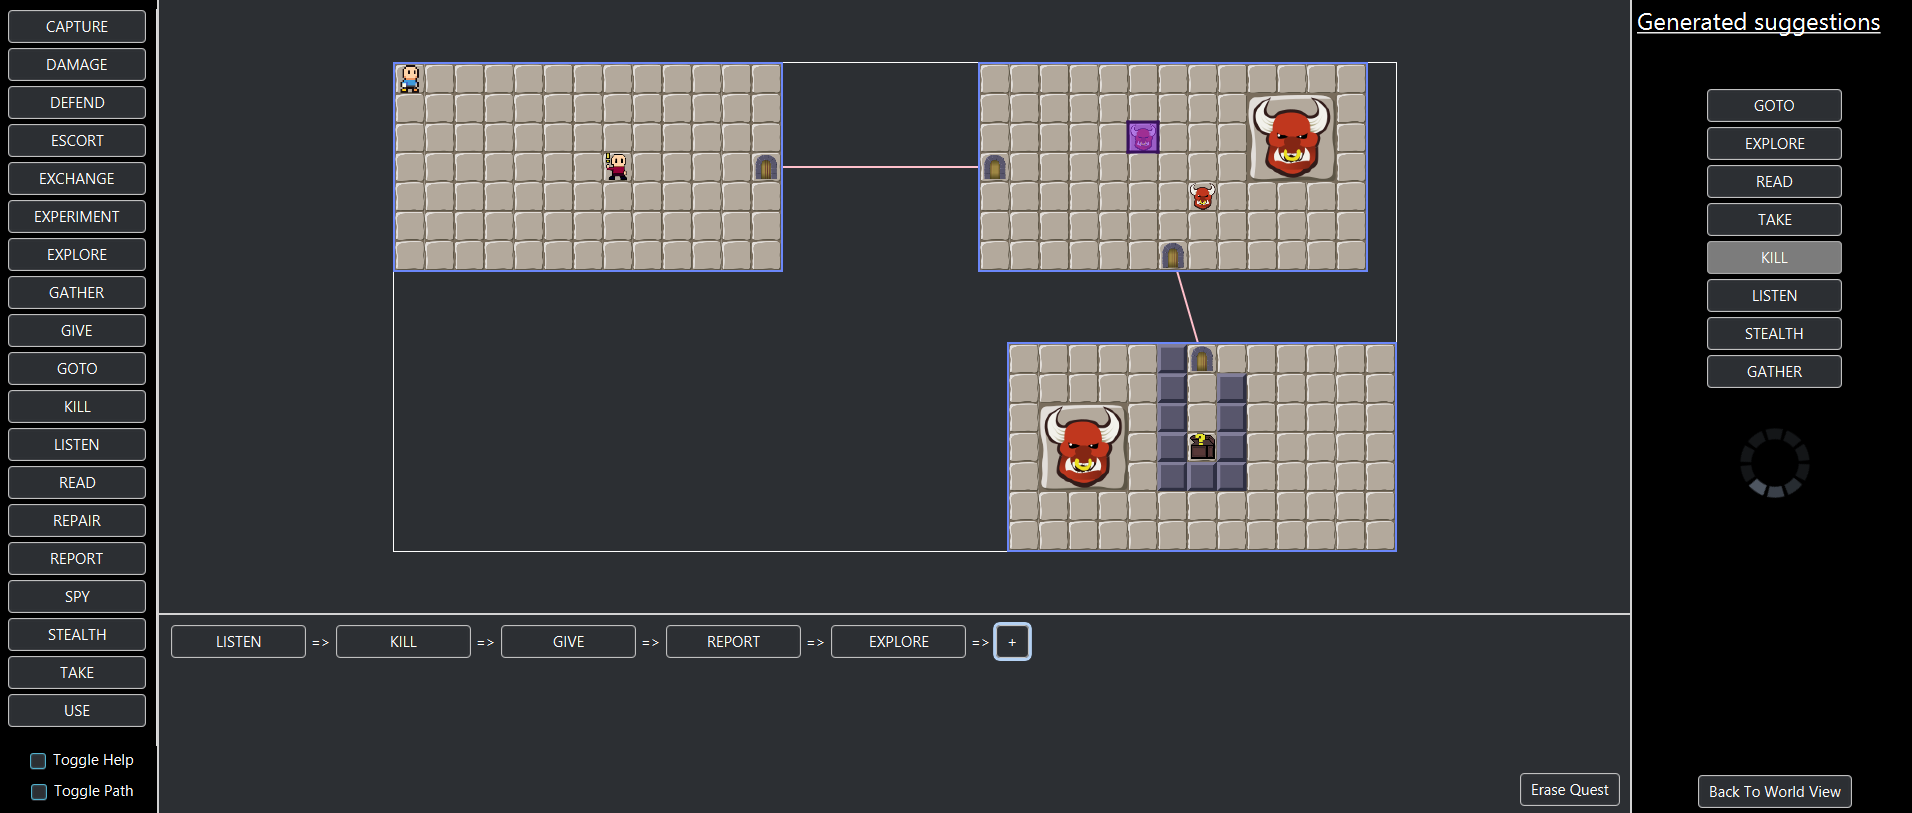
\includegraphics[width=1\textwidth]{included-papers-tex/paper-8/figures/main-sug.png}
        \caption{An example quest sequence and the user attempting to select a suggested quest action}
        \label{figs:GUI:suggestions}
    \end{subfigure}
    \begin{subfigure}[t]{0.48\textwidth}
        \centering
        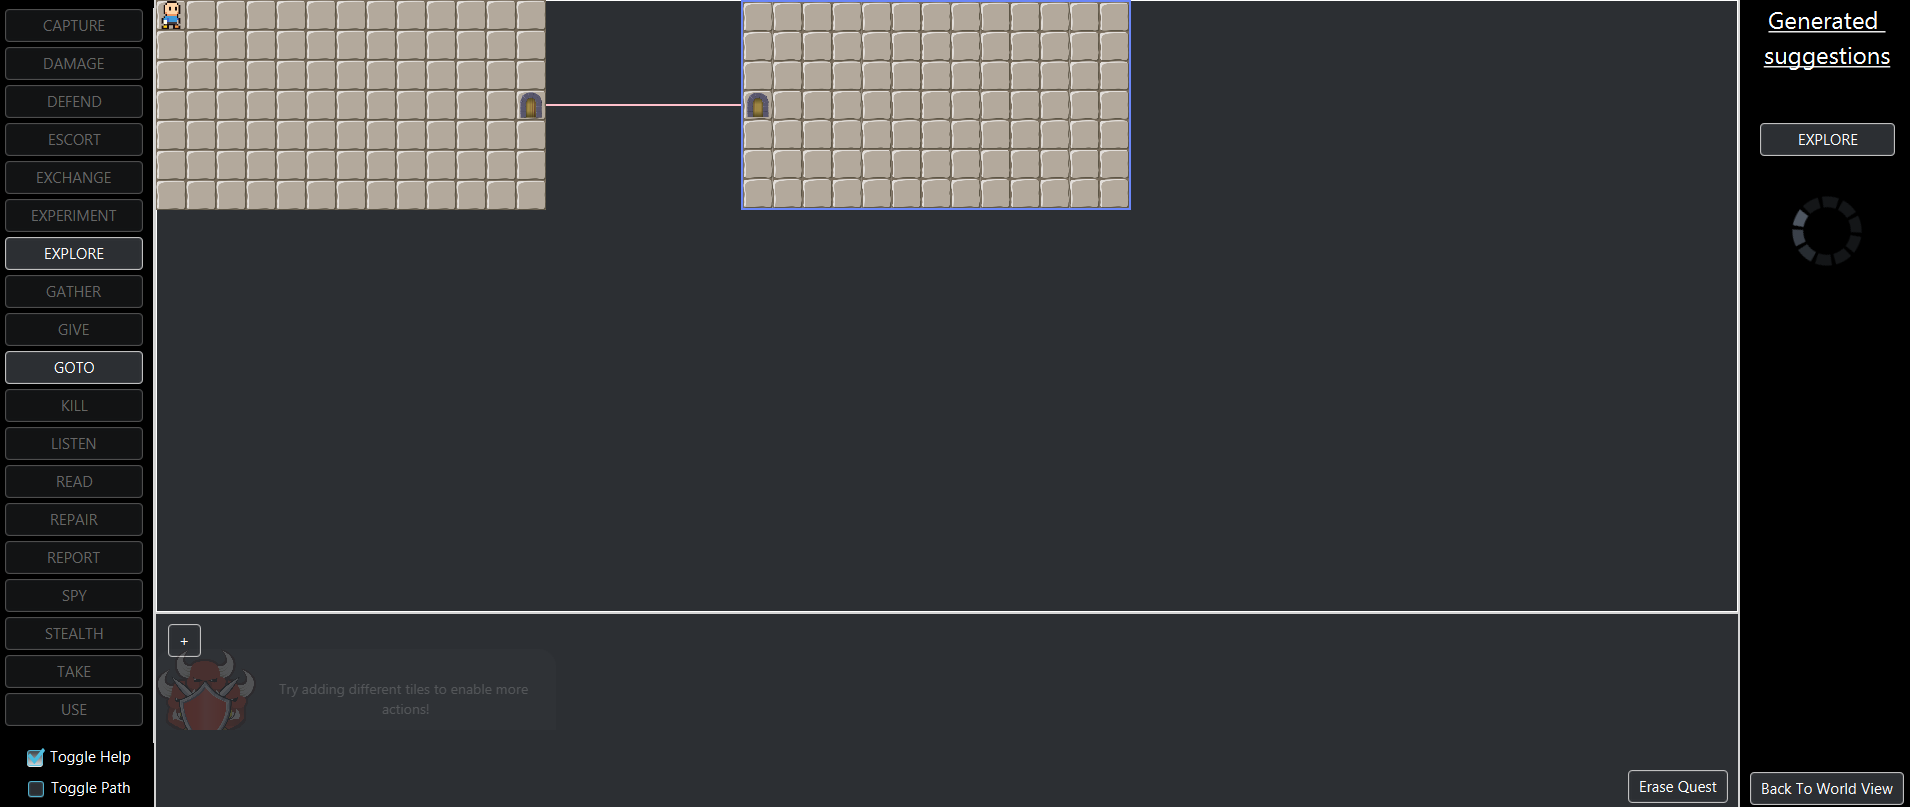
\includegraphics[width=1\textwidth]{included-papers-tex/paper-8/figures/main-available-quest.png}
        \caption{Example of two empty and connected rooms, where most prerequisites for quest actions are not met.}
        \label{figs:GUI:avQuest}
    \end{subfigure} \hfill%
     \begin{subfigure}[t]{0.48\textwidth}
        \centering
        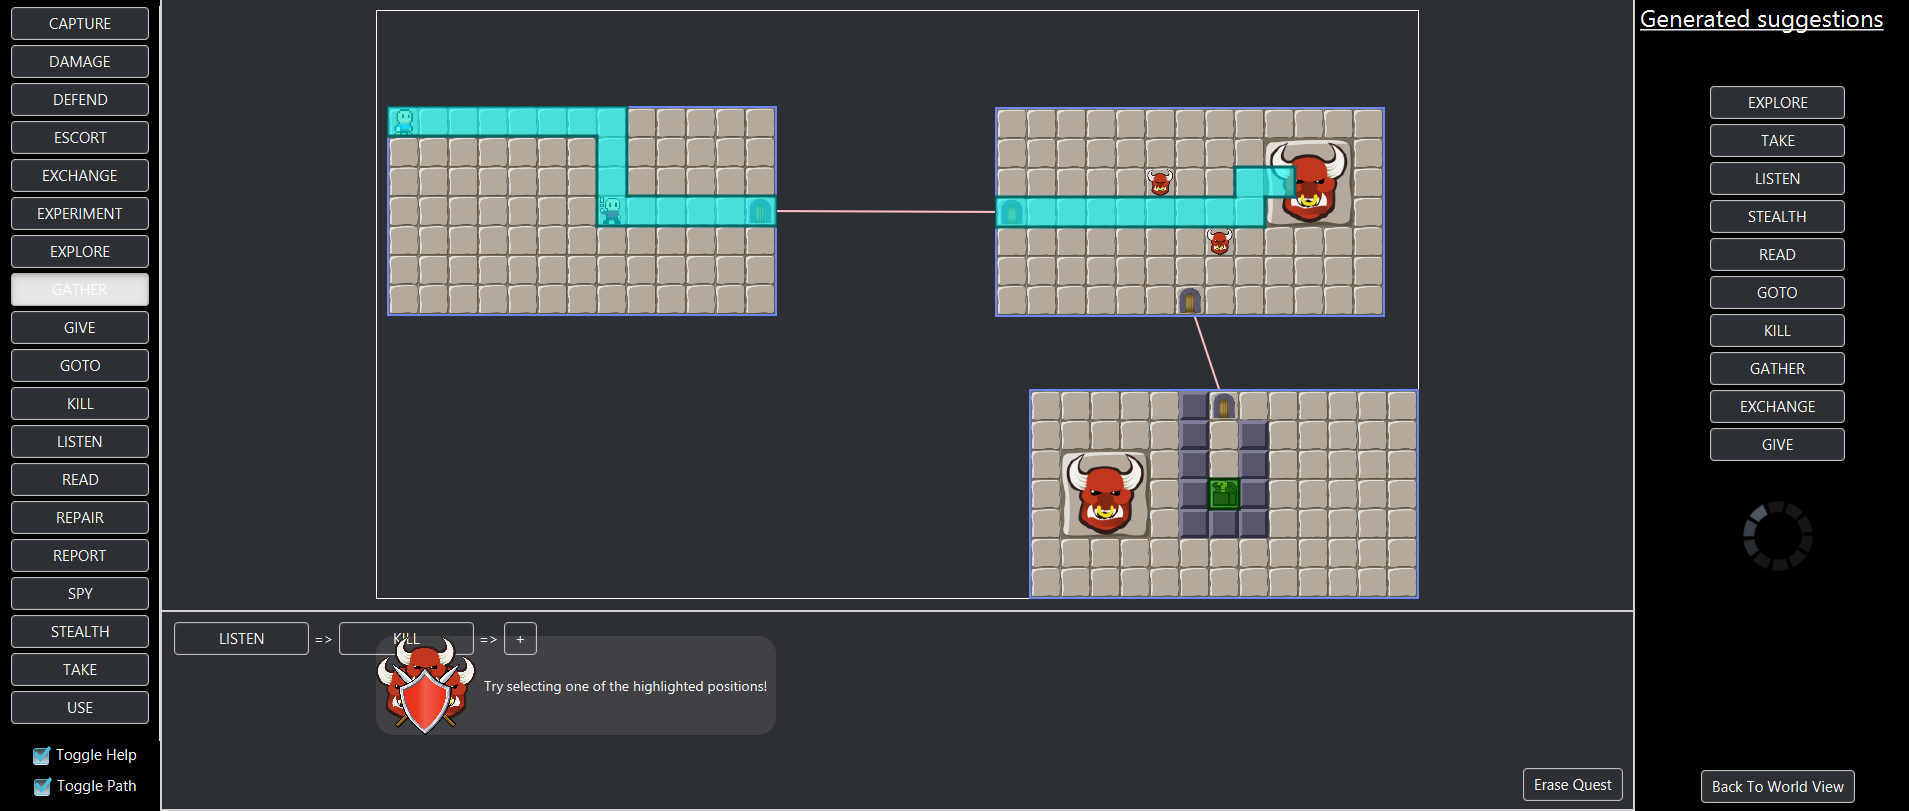
\includegraphics[width=.99\textwidth]{included-papers-tex/paper-8/figures/main-help.png}
        \caption{Example of the provided help for designers. A pop-up informs them of events, and in cyan, the A* path.}
        \label{figs:GUI:help}
    \end{subfigure}%
     \begin{subfigure}[t]{0.48\textwidth}
        \centering
        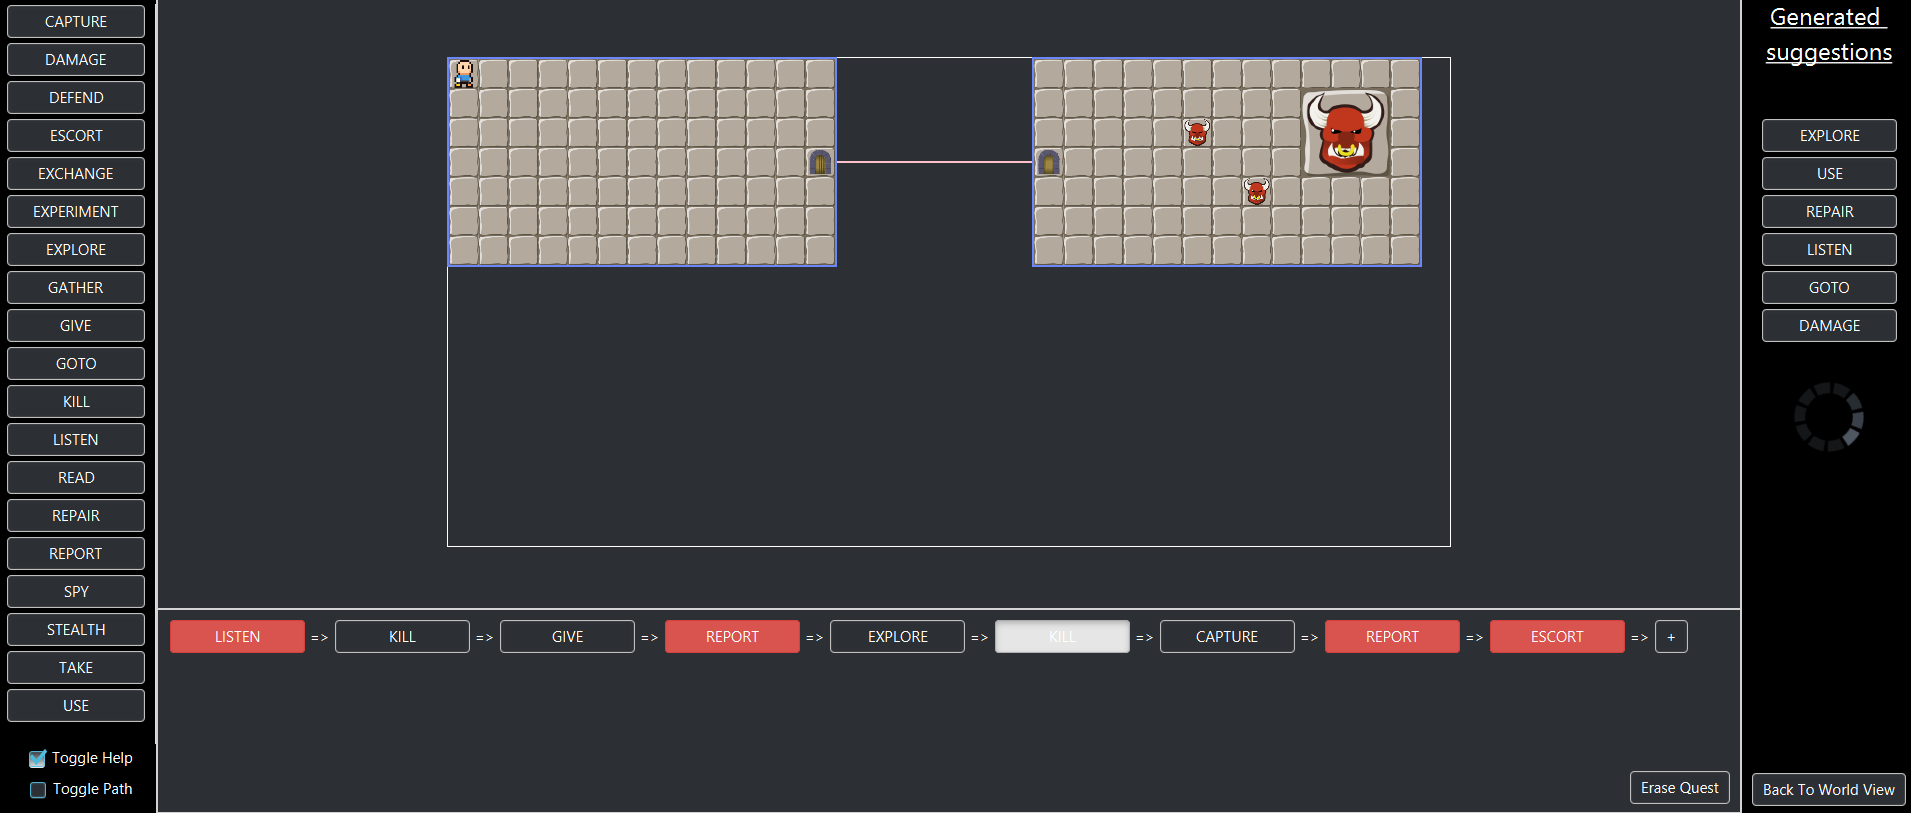
\includegraphics[width=.99\textwidth]{included-papers-tex/paper-8/figures/main-errorQ.png}
        \caption{Error in the quest sequence since the designer erased a room containing quest action tiles.}
        \label{figs:GUI:error}
    \end{subfigure} \hfill%
    \caption{Visualization of the GUI used for creating quest sequences and different states}
    \label{figs:GUI}
\end{figure*}

Questgram is a quest generation tool that lets the designer compose one long sequence of quest actions to create an overarching objective for the dungeon they are creating. These quest actions are based on the quest analysis and classification and produced grammar by Doran and Parberry~\cite{p8Doran2011-questsMMORPGs}. Questgram builds on top of EDD extending its level design and generation capabilities with a mixed-initiative quest editor and takes advantage of its mixed-initiative perspective and the level design system.


% , where a set of nine NPC motivations were extracted, and formed as a production rules for a grammar. Our system is implemented on top of EDD, extending its level design and generation capabilities with a mixed-initiative quest editor. 

%Therefore, EDD needed to be extended with some key elements such as a new quest editor view and new tiles such as and NPC (i.e., quest giver)

% Following Yu et al. formal definition, each quest action would be a task $t$, which is represented by a 4-tuple $\langle C, M, I, R_{t} \rangle$, where $C$ are the game elements created by the designer linked to a quest action as described in table~\ref{table:prereq} and the grammar itself. $M$ is the level editor in EDD. $I$ is partially disregarded as the quest are not presented to players, but integrated as a sequence list shown in figure~\ref{figs:GUI:overview}. Lastly, as the system creates an overarching quest rather than $R_{t}$ is implicitly incorporated when set

% Following Yu et al. formal definition, a quest in Questgram is a long sequence of quest actions or tasks that must be fulfilled sequentially. 

%Perhaps some formal definition?

EDD was extended with some key elements such as a new quest editor view depicted in figure~\ref{figs:GUI:overview}, and two new generic tiles; an NPC acting as quest giver and target, and a quest item, which is the subject of many quests. These two new tiles were kept as generic as possible for future systems to have the responsibility of handling what type of NPC and object should replace those, similarly as with the other tiles in EDD such as the generic enemy, boss, and treasure. These tiles, together with the pre-existing enemy and boss tiles, have been intertwined with the actions, resulting in the "unlocking" mechanism of different quests, which can be observed in table~\ref{table:prereq}. It must be noted that while Questgram integrates and utilizes the different features and tiles of EDD's level generation facet, there is no integration of the new tiles and quests with EDD's evolutionary algorithm IC MAP-Elites~\cite{p8Alvarez2020-ICMAPE}. This is left for future work.

While games can be either linear, semi-open, or open, with branching narratives and the design structured by the types of quests featured in a game~\cite{p8aarseth2005hunt}, with concepts such as kernels and satelites~\cite{p8Aarseth2012-Narrativetheory}; our approach only allows for the creation of a single overarching quest.

% our system forces the game to be linear. 

% Furthermore, our approach only let designers create one single overarching quest, which can be seen as a set of subquests.

% One limitation of our system is that it only allows for a single overarching quest, which can be seen as a set of quests, 

% While games can be either linear, semi-open, or open, and the design is structured by the types of quests featured in a game~\cite{p8aarseth2005hunt}, with concepts such as kernels and satelites~\cite{p8Aarseth2012-Narrativetheory}; our system forces the game to be linear. 

\subsubsection{Quest Actions}

% Please add the following required packages to your document preamble:
% \usepackage{graphicx}
\begin{table*}[]
\caption{displaying the actions together with Doran and  Parberry's~\cite{Doran2011-questsMMORPGs} prerequisites and how the actions and the previously mentioned prerequisites have been implemented in EDD. This indirectly explains the “unlocking” - describing what tiles that must be placed for an action to be available. Note that “Goto” \& “Explore” do not have any special tile prerequisites besides available floor. }
\label{table:prereq}
\resizebox{\textwidth}{!}{%
\begin{tabular}{lll}
\hline
Action   & Prerequisites in~\cite{Doran2011-questsMMORPGs} & Prerequisites in EDD \\ \hline
Capture    & “Somebody is there”                          & A NPC or boss/enemy must be placed.                        \\
Damage     & “Somebody or something is there”             & An item or NPC must be placed.                             \\
Defend     & “Somebody or something is there”             & An item or NPC must be placed.                             \\
Escort     & “Somebody is there”                          & A NPC must be placed.                                      \\
Exchange & “Somebody is there, they and you have something”          & A NPC and an item must be placed (requires two positions). \\
Experiment & “Something is there”                         & An item must be placed.                                    \\
Explore    & “none”                                       & An available floor tile.                                   \\
Gather     & “Something is there.”                        & An item must be  placed.                                   \\
Give       & “Somebody is there, you have something.“     & A NPC and an item must be placed (requires two positions). \\
Goto       & “You know where to go and how to get there.“ & An available floor tile.                                   \\
Kill       & “Somebody is there.“                         & A boss/enemy must be placed.                               \\
Listen     & “Somebody is there.“                         & A NPC must be placed.                                      \\
Read       & “Somebody is there.“                         & A NPC must be placed.                                      \\
Repair     & “Somebody is there.“                         & A NPC must be placed.                                      \\
Report     & “Somebody is there.“                         & A NPC must be placed.                                      \\
Spy        & “Somebody or something is there.“            & A NPC or boss/enemy must be placed.                        \\
Stealth    & “Somebody is there.“                         & A NPC or boss/enemy must be placed.                        \\
Take       & “Somebody is there, they have something.“    & A NPC and an item must be placed (requires two positions). \\
Use        & “There is something there.“                  & An item must be placed.                                    \\ \hline
\end{tabular}%
}
\end{table*}

\begin{table}[]
\caption{displaying the grammatical rules. The columns marked with asterisks are identified as “motivations” by Doran and Parberry~\cite{Doran2011-questsMMORPGs}, but are used as a starting point for the quests. The “\textless \textgreater{}” indicates the next production rule to be taken, and actions without “\textless \textgreater{}” is  the terminating action.}
\label{tab:productionRules}
\resizebox{\textwidth}{!}{
\begin{tabular}{ll}
\hline
Production   rules &
  Actions \\ \hline
knowledge* &
  {[}"\textless{}get\textgreater{}","\textless{}go\_to\textgreater{}","give"{]},   {[}"\textless{}spy\textgreater{}"{]}, \\
  &
  {[}"\textless{}go\_to\textgreater{}","listen","\textless{}go\_to\textgreater{}","report"{]}, \\
 &
  {[}"\textless{}get\textgreater{}","\textless{}go\_to\textgreater{}","use","\textless{}go\_to\textgreater{}","give"{]} \\
comfort* &
  {[}"\textless{}get\textgreater{}","\textless{}go\_to\textgreater{}","give"{]},\\
  &
  {[}"\textless{}go\_to\textgreater{}","damage","\textless{}go\_to\textgreater{}","report"{]} \\
reputation* &
  {[}"\textless{}get\textgreater{}","\textless{}go\_to\textgreater{}","give"{]},   \\
 &
 {[}"\textless{}go\_to\textgreater{}","\textless{}kill\textgreater{}","\textless{}go\_to\textgreater{}","report"{]}, \\
 &
  {[}"\textless{}go\_to\textgreater{}","\textless{}go\_to\textgreater{}","report"{]} \\
serenity* &
  {[}"\textless{}go\_to\textgreater{}","damage"{]},   \\
 &
 {[}"\textless{}get\textgreater{}","\textless{}go\_to\textgreater{}","use","\textless{}go\_to\textgreater{}","give"{]}, \\
 &
  {[}"\textless{}get\textgreater{}","\textless{}go\_to\textgreater{}","use","capture","\textless{}go\_to\textgreater{}","give"{]}, \\
 &
  {[}"\textless{}go\_to\textgreater{}","listen","\textless{}go\_to\textgreater{}","report"{]},   \\
 &
 {[}"\textless{}go\_to\textgreater{}","take","\textless{}go\_to\textgreater{}","give"{]}, \\
 &
  {[}"\textless{}get\textgreater{}","\textless{}go\_to\textgreater{}","give"{]},   \\
 &
 {[}"\textless{}go\_to\textgreater{}","damage","escort","\textless{}go\_to\textgreater{}","report"{]} \\
protection* &
  {[}"\textless{}go\_to\textgreater{}","damage","\textless{}go\_to\textgreater{}","report"{]},   \\
 &
 {[}"\textless{}get\textgreater{}","\textless{}go\_to\textgreater{}","use"{]}, \\
 &
  {[}"\textless{}go\_to\textgreater{}","repair"{]},   {[}"\textless{}get\textgreater{}","\textless{}go\_to\textgreater{}","use"{]},   \\
 &
 {[}"\textless{}go\_to\textgreater{}","damage"{]}, {[}"\textless{}go\_to\textgreater{}","repair"{]}, \\
 &
     {[}"\textless{}go\_to\textgreater{}","defend"{]} \\
conquest* &
  {[}"\textless{}go\_to\textgreater{}","damage"{]},   {[}"\textless{}go\_to\textgreater{}","\textless{}steal\textgreater{}","\textless{}go\_to\textgreater{}","give"{]} \\
wealth* &
  {[}"\textless{}go\_to\textgreater{}","\textless{}get\textgreater{}"{]},   {[}"\textless{}go\_to\textgreater{}","\textless{}steal\textgreater{}"{]}, {[}"repair"{]} \\
ability* &
  {[}"repair","use"{]},   {[}"\textless{}get\textgreater{}","use"{]}, {[}"use"{]},   {[}"damage"{]}, \\
 &
  {[}"\textless{}get\textgreater{}","experiment"{]} \\
equipment* &
  {[}"repair"{]},   {[}"\textless{}get\textgreater{}","\textless{}go\_to\textgreater{}","give"{]},   {[}"\textless{}steal\textgreater{}"{]},\\
 &
  {[}"\textless{}go\_to\textgreater{}","exchange"{]} \\
subquest* &
  {[}"\textless{}go\_to\textgreater{}"{]},   {[}"\textless{}go\_to\textgreater{}","\textless{}QUEST\textgreater{}","go\_to"{]} \\
go\_to &
  {[}"explore"{]},   {[}"\textless{}learn\textgreater{}","go\_to"{]} \\
learn &
  {[}"\textless{}go\_to\textgreater{}","\textless{}subquest\textgreater{}","listen"{]},   \\
 &
 {[}"\textless{}go\_to\textgreater{}","\textless{}get\textgreater{}","read"{]}, \\
 &
  {[}"\textless{}get\textgreater{}","\textless{}subquest\textgreater{}","give","listen"{]} \\
get &
  {[}"\textless{}steal\textgreater{}"{]},   {[}"\textless{}go\_to\textgreater{}","gather"{]}, \\
 &
  {[}"\textless{}go\_to\textgreater{}","\textless{}get\textgreater{}","\textless{}go\_to\textgreater{}","\textless{}subquest\textgreater{}","exchange"{]} \\
steal &
  {[}"\textless{}go\_to\textgreater{}","stealth","take"{]},   {[}"\textless{}go\_to\textgreater{}","\textless{}kill\textgreater{}","take"{]} \\
spy &
  {[}"\textless{}go\_to\textgreater{}","spy","\textless{}go\_to\textgreater{}","report"{]} \\
capture &
  {[}"\textless{}get\textgreater{}","\textless{}go\_to\textgreater{}","capture"{]} \\
kill &
  {[}"\textless{}go\_to\textgreater{}","kill"{]} \\ \hline
\end{tabular}
}
\end{table}

Doran and Parberry identified 19 different actions to be used as quest actions~\cite{p8Doran2011-questsMMORPGs}, which we implemented and where each has its contextual prerequisites to be able to add them. In some cases, we have decided regarding if the actor represented in the action is friendly, e.g., NPC, or hostile, based on the tool's nature and the levels created. These actions are available for both the grammar and the designer to create as many steps as wanted in the overarching quest. The actions, their original prerequisite, and the domain-specific prerequisite are depicted in table~\ref{table:prereq}. 

These actions can be added one after each other in any order by the designers allowing for combinations and quests outside of the possible grammar seen in table~\ref{tab:productionRules}. Besides manual creation, the designer can instead pick a suggested action from the generated actions from the right panel, which offers the next action to be added to the quest. After deciding these options, the user will need to press the "+" button on the bottom panel, which will add the action to the quest sequence.


% Based on Doran and Parberry's work, we implemented 19 different actions to be used as quest actions~\cite{p8Doran2011-questsMMORPGs},. In some cases, we have made the decision regarding if the actor represented in the action is friendly e.g., NPC or hostile e.g., enemy given the nature of the tool and the levels created. These actions are available for both the grammar and the designer to create as many steps as wanted in the overarching quest.  The actions are depicted in table~\ref{tab:prerequisites}, which also shows 

% These actions can be added one after the other one in any order by the designers allowing for combinations and quests outside of the possible grammar seen in table~\ref{tab:grammar}

% In order for designer to add some actions, they require some prerequisites 

% 19 different actions have been added to the quest implementation. These are based on Parberry and Dorans research [8]. However in some cases, we have made the decision regarding if the actor represented in the action is friendly (NPC) or hostile (enemy), this will be evaluated in the user feedback.  The actions have different prerequisites (table 1). With the actions “unlocking” through the user placing the necessary tiles. The user has the option to select what type of action and then what position on the map the action will take place. This is done by selecting a specific floor tile, marking that position on the map. However, Exchange, Give, and Take requires two positions due to its two subject nature (an actor + an item). 

% Besides manual placement, the user has the option to instead pick a suggested action from the generated actions from the right panel. After deciding these options, the user will need to press the “+” button on the bottom panel, this will add the action to the quest sequence

\subsubsection{Quest Grammar}

The system employs a generative grammar, specifically Lindenmayer Systems (L-Systems)~\cite{p8Lindenmayer1996-LSystems} to generate the different set of quests using the production rules depicted in table~\ref{tab:productionRules}. The production rules are divided into two categories: 1) motivations for NPCs to start a quest such as~\emph{knowledge} where the focus would be to create quests with more passive actions or~\emph{reputation} where the focus would be to kill some enemy to gain reputation with some NPC. 2) Non-motivation rules related to the development of quests (i.e., non-terminal symbols) such as "go\_to" or "get". In table~\ref{tab:productionRules} non-terminal symbols are represented with "<" and ">", and terminal symbols simply list the action.

% The system can generate complete quests on its own by using one of the NPC Motivations as axiom, but when used in a mixed-initiative fashion with the designer manually creating the quests, the system uses the current active quest sequence created by the designer. The system then proposes a set of valid quest items to the designer to continue the quest or replace a current action. 

The system can be used for generating complete quests on its own, which select one of the NPC motivations as an axiom or with the designer in a mixed-initiative approach. As a mixed-initiative approach, the designer can manually create a quest sequence while the system uses the current quest sequence to suggest a set of valid quest items to the designer to continue the quest or replace a current action. Given that the production rules are invariable, there can be situations where the system cannot generate quests based on the quest sequence. This would result in the designer receiving feedback that the quest is not compatible with the grammar itself, giving the designer suggestions on how to continue and overcome this limitation.

Quest actions are suggested to continue the current sequence and append a new action at the end, or they can be used to replace an action in any position of the current sequence. For both, the system continuously produce quests using the grammar and filters out those that do not match the designer's sequence up to the position where they wish to change a quest action. In this way, the designer can choose suggestions for either continuing and finishing the quest or replacing existing parts for other valid actions.

% In the latter, the sequence up to the position where the designer wishes to change a quest action 

% change an action is used as axiom of the quest generator. In this way, the designer is given the option to choose suggestions for either continuing and finishing the quest or replace existing parts for other valid actions.

% Through this, the quest sequence might become unusable for the grammar to produce new suggestions, given that a sequence might not exist, but since the . We acknowledge this as a limitation of the system

\subsubsection{Workflow}

The GUI for the quest generation system of EDD follows the same concept and design as the room editor for consistency. Placeable quest actions are at the left pane, and generated suggestions with the grammar are at the right pane. The whole dungeon can be seen on the center top pane, and at the center bottom, the designer can compose the quest. These parts can be explicitly seen in figure~\ref{figs:GUI:overview}.

The designer cannot add any quest action, which prerequisite has not been fulfilled yet as described in table~\ref{table:prereq} and exemplified in figure~\ref{figs:GUI:avQuest}. Quest actions need to be linked to some actual tile representation in the dungeon. For instance, a "KILL" action requires selecting an enemy, while the "GO TO" requires any floor tile. Therefore, once the designer adds a new quest action, they must choose which tile is linked to this, presented to the designer in green. Similarly, when a quest action is suggested, the system randomly picks an available tile shown in purple to the designer as shown in figure~\ref{figs:GUI:suggestions}.

Moreover, the sequence panel is displayed in fig. 7.4. The panel displays the actions the user has selected. To add a sequence to the list, the user needs to manually select an action and its desired position or select a suggested action. Both of these options require the user to press the "+" button manually. Similarly, each quest action in the sequence is clickable and interchangeable. If a quest action in the sequence is selected, the designer can exchange it by selecting the quest action desired from the action panel or from the newly suggested actions, or remove it.

Finally, the designer can toggle two different types of assistance. The first focuses on informing the designer of changes in the sequence due to a manually placed or automatically generated, and informs the designer of the tile that needs to be selected. The second assistance shows A* paths between the target tile of a selected quest action and the next target tile. Both assistance is depicted in figure~\ref{figs:GUI:help}.

% The user interface for quest-tool implementation follows the room-view’s design, and consists of four panels; the left-hand toolbar, the right-hand generated suggestions, the central map-view, and the bottom quest-panel (fig. 7).

% 4.3.2.1 Action tiles

% Since EDDs world map is reused in the quest tools, all of EDDs pre-existing visual elements remain the same in the quest view. An action takes up 1x1 square which is the general size of tile elements in EDD, however a boss requires 4x4 tiles, though this is still treated as 1x1 entity, and thus an 1x1 tile of the 4x4 is required to be selected. Once an action is placed on the room manually, the available tiles where the action can be placed will be displayed in green (fig. 2). When the user selects a suggestion from the generator, the available tiles will instead be displayed in purple (fig. 3). 
  
% Figure 2 displaying an user manually selecting the “listen” action, therefore the NPC will be highlighted in green to display its availability.

% Figure 3 displaying a user selecting a generated suggestion, “give”, the generator automatically selects the required tiles and highlights them in purple. 

% 4.3.2.2 Action panel

% The action panel is displayed in fig. 7.1. The panel consists of buttons for each respective action (19 actions). The tile placed in the room reflects the available actions, which is previously discussed in section 4.1.2. This panel represents the manual placements and manual aspect of the mixed initiative approach of the tool. If an action is not “unlocked” based on the prerequisites, it is disabled and the button is colored a dark gray. If an action fulfills its prerequisites it is enabled and turns light gray and white borders and text (fig. 4).

% Figure 4 displaying two rooms with no added tiles. Since ”goto” and “explore” only requires a floor tile, it is “unlocked” and therefore enabled. The rest of the buttons are “locked” and therefore displayed as the same color as the background.

% 4.3.2.3 World panel

% The world panel is displayed in fig. 7.2. 

% The panel displays the reused EDD world view. The world view displays the user’s dungeon and the tiles placed. The selected actions will be visible on the map (fig. 2). 

% 4.3.2.4 Suggestion panel

% The suggestion panel is displayed in fig. 7.3. The panel displays the generated actions from the generator. Once the generator generates a suggestion, it will be displayed in a list. The list is clickable, and once an action is selected it is highlighted in a lighter gray (fig. 5). To add the generated suggestion to the quest sequence, the user needs to click on the “+” symbol, therefore adding it on either last place or the desired place in the sequence. While the generator is “working”, a loading symbol is displayed, indicating to the user to wait. 

% 4.3.2.5 Sequence panel

% The sequence panel is displayed in fig. 7.4. The panel displays the actions the user has selected. In order to add a sequence to the list, the user either must manually select an action and its desired position, or select a suggested action, however both these options require the user to manually press the “+” button. 

% Each button in the sequence is clickable and interchangeable. If an action in the sequence is selected, the user can select the action desired from the action panel to be exchanged. When an action button is selected, removal is done by pressing delete on the user’s keyboard.

% 4.3.2.6 Toggle Menu

% The toggle menu is displayed in fig. 7.5. The menu consists of two buttons, toggle help and toggle path. 
% Enabling toggle help results in several help dialogs being displayed for the user. The dialog informs the user that a placement must be picked in a room, but in addition informs the user that a certain action was added to the sequence. The alerts fade and disappear after 4.5 seconds. 

% Toggle path displays the shortest path from the user’s characters through all placed positions to the recent placed. This is done through a modified Dijkstra's algorithm. The path is displayed in light blue (fig. 6).  
 
% Figure 5 displaying a dialog message informing the user to pick a position in the room.
 
% Figure 6 displaying the shortest path from the character (left corner) to a “goto” action (recent action) placed in the next room.

% 4.3.2.7 Erase and Back 

% The button “erase” and “back” is displayed in fig. 7.6 and 7.7. “Erase” erases the quest sequence while “back” directs the user to the world view (fig 1).

% \subsection{Concepts and Definitions}

%This paper presents an approach and fundamental steps towards the implementation of designer personas: an analysis of designer style clustering to isolate archetypical paths that can be later be used to build ML surrogate models of archetypal designers. Such models would adapt to the dynamic designer during the mixed-initiative creative process by being placed in the solution space, allowing the designer to traverse such space of models as she drifts through the many dimensions of her creative process.

% design archetypes 

Our work draws from ideas, concepts, and definitions introduced by Liapis et al., such as the core designer model loop when using CAD tools, what can be modeled: preferences, style, goals, processes, and their definition, and particularly, the use of designer modeling as an individual or collective model~\citeptenth{p10Liapis2013-designerModel}. We support our approach on the idea of style as a particular type of designer's preference, and that a collective model can be used to form a stable and static design space, which after being interacted with by designers, can be adapted towards them.

% and the idea of style as a particular type of designer's preference.

%. Moreover, Liapis et al. discuss the modeling of style as a type of preference, where each individual designer has peculiarities and characteristics that makes their style recognizable. While we agree with this vision, we 

%Our work draws from many of the ideas and concepts introduced by Liapis et al.~\citeptenth{p10Liapis2013-designerModel}, in relation to style, goals, preferences and design processes of designers. Nevertheless, given the interdisciplinary scope of this system, and the multiple concepts discussed throughout the paper, it is essential to have operational definitions on the different terms used.

%Thus, in this paper, the shared goal is set and defined by the designer with her design, and as she develops, adapts, and changes, the system seeks to adjust its goals to support the designer's work. Furthermore, the aim of this paper is to propose a system that is able to identify the designer's current goal and style to adapt further the system's goals to provide a personalized experience.

\subsubsection{Design Style} \label{sec:designStyle}

%Every designer has a different style when creating content, especially levels, where one might 

% One idea is to train a supervised learning model on traces of other collaborative creation session and try to predict the next step the human would take in the design process. The main problem with this is that people are different, and different creators will want to take different design actions in the same state;

% One way of overcoming this problem could be to change the level of abstraction at which design actions are modeled and predicted. Instead of predicting individual edits, one could identify different styles or phases of the artifact being created, and model how a designer moves from one to another. To put this concretely in the context of designing rooms for a Zelda-like dungeon crawler~\citeptenth{p10tloz}, one could classify room styles depending on whether they were enemy onslaughts, complex wall mazes, treasure puzzles, and so on. One could then train models to recognize which types of rooms a user creates in which order. By clustering sequences of styles or phases we could formulate designer personas as archetypical trajectories through style space, rather than as sequences of individual edits. For example, in the context of creating a dungeon crawler, some designers might start with the outer walls of the rooms and then populate it with NPCs, whereas another type of designer might first sketch the path they would like the player to take from the entrance to the exit and then add parts of the room outside the main path.

There exist many different styles when creating content, especially levels, that designers can create and adapt to accomplish their goals and the experiences they want for players. On a general level, \emph{Design Style} encompasses the creative process from conceptualization, prototyping, reflection, adaptation, especially when following different processes or constraints during collaboration. Taking a more concrete and operational level, \emph{Design Style} can be analyzed as overarching goals that different designers have when creating a dungeon. For instance, dungeons in games such as Zelda\citeptenth{p10tloz} or The Binding of Isaac\citeptenth{p10mcmillen_binding_2011}, represent a particular playing style planned by the designer. In the former, low tempo, exploring the dungeon, and secret rooms define the style of the dungeons, whereas in the latter, high tempo, optimizing time and resources, small rooms, and in general high-challenge define the dungeons. 

While interesting and relevant to understanding the designers' holistic design process and the expected player experience, \emph{Design Style} can also be discussed on an individual room basis. Rooms have their own set of characteristics and styles that can be identified and modeled to understand their design process. Some would prefer to create the room's architecture first to then create the goals within, whereas others would like to place strategic objectives around and then create the architecture around it or alternating between both. Even with such a division, how to reach those design styles is not straightforward and does not require the same strategy, which also shows the preference and style of individual designers. For instance, if the goal is to create a challenge to reach a door, the designer could create a room with a substantial number of enemies, create a concentrated high-challenge in the center of the room, or divide the room into smaller choke areas. Therefore, in this paper, we take a simplified view of \emph{Design Style} and treat it as the style designers follow to create a room, informed by the individual steps each has taken connected to their preferences and goals.

% While this is a simplified view of \emph{Design Style}, we acknowledge that this is a simplified view of \emph{Design Style}, as this could encompass 

% I take some issue with the framing of the paper as being one of modeling someone’s “design style” based only on the sequence of design actions taken as evidenced in snapshots of a design process. To be clear, I think the snapshot approach is a perfectly reasonable one.  But I worry that giving it a term as all-encompassing as “design style” is overpromising, because there is so much about someone’s approach to design that is lost in reducing it to a sequence of partial designs: moments of self-reflection, prototyping and throwing away ideas before moving to new ones, experimentation on paper away from the machine, prior exposure to design and how it informs new design choices, adherence to norms of genre. Obviously these cannot be captured through this approach, nor do they need to be for the work to be valid. Nonetheless, it seems unfair to characterize “design style” as a mere sequence of edit operations.

% I think more precise language would also make clearer what the strengths and limitations of this study are. By naming the aspects of design that are not captured, it makes clear what potential future work there is, how this approach should and should not be applied in other design tools, and the extent to which this work may be generalizable across tools and genres.

% I think this issue also comes up in cluster labeling. Some of the cluster labels refer to properties of room layout (e.g. “maze-like complex architecture”; “dense room”), some to meta-aspects of design (e.g. “high challenge, clear goal”), some to types of actions (e.g. “separating and populating chambers”, “balancing and optimizing”). It seems like it should be possible for a room to fall into two of these labeled clusters simultaneously (e.g. a maze-like room that has many enemies and a clear goal at the end of the maze), and it’s confusing that these are separate clusters. The same is true for other cluster pairs (e.g. “bordered rooms with deeper architectural development” and “dense, full-range leniency” seem like they could co-exist). It’s also not clear how these cluster labels are applied (other than a “qualitative analysis” — but was this done by the research team, or by external experts? how was this evaluated?).


% we use a simplified vision of \emph{Design Style}

% this general level is interesting to udnerstand the designer's holistic design process, there is a need to 

% analyzing the individual rooms gives a

% Every designer has a different style when creating content, especially levels, some would prefer to create the architecture of the room first to them proceed to create the goals within, whereas others would like to place strategic objectives around and then create the architecture around it or alternating between both. Even with such a division, how to reach those design styles is not straightforward and does not require the same strategy, which also shows the preference and style of individual designers. For instance, if the goal is to create challenge to reach a door, the designer could create a room with a substantial amount of enemies, or create a concentrated high-challenge in the center of the room, or divide the room into smaller choke areas.

% Going to a more general level, one could also think of the designs as overarching goals that different designers have when creating the dungeon. For instance, dungeons in games such as Zelda\citeptenth{p10tloz} or The Binding of Isaac\citeptenth{p10mcmillen_binding_2011}, represents a certain playing style planned by the designer. In the former, low tempo, exploring the dungeon, and secret rooms defines the style of the dungeons, whereas in the latter, high tempo, optimizing time and resources, small rooms, and in general high-challenge. While this general level is interesting to udnerstand the designer's holistic design process, there is a need to 

% the whole dungeon represents a certain playing style the design

% One can also think on the designs as a overaching goals that different designers would have, some would luike a high-tempo with smaller rooms and high challenge with minimal rewards while others might prefer the designer to go through more convoluted mazes with many connections to confuse the player and reward the understanding of patterns. While this view is interesting to understand the designer's holistic design process; in this paper we threat Design Style specifically as the style designers follow to create a room, informed by the individual steps each has taken.


% % I think i should discuss 

% % While very discussed, style 

% We can discuss this in both a specific and general level. For adventure and rogue-like games such as Zelda\citeptenth{p10tloz} or The Binding of Isaac\citeptenth{p10mcmillen_binding_2011}, the whole dungeon represents a certain playing style the design  %in-development

% \subsubsection{Designer's Goals}

% Usually, designers' goals are linked to the experiences they want to create for players, however, in a MI-CC tool, the goal is defined as the 

% It is identified as the 
% The designer's goal is defined as the current state of rooms and the set of interactions done in the tool or sequence of steps taken thus far, to reach such a state. Goals by the designer are linked to the addition and strategic placement of enemies and treasures, giving some goal for the player, e.g., forcing the fight with an enemy or allowing the player to avoid the conflict through side paths.



%Specifically, this definition is used as the current goal to be achieve by the designer identified as the sequence of steps taken thus far. Goals by the designer are linked to the addition and strategic placement of enemies and treasures, which gives some type of goal for the player, e.g. force the fight with an enemy or give the opportunity for the player to avoid the conflict through side paths. 

%Moreover, in EDD the designer is tasked to create a dungeon with an unlimited amount of interconnected rooms where each room can be further designed on it's own. When designing the dungeon and the rooms, the designers have the freedom to create the rooms as they want with any goal for the player. For instance, if the goal of the designer is to create a boss room, she might create a room with some narrow corridors that end up in a fight with a boss.



% \subsubsection{System Goals}

% The system goals are defined as the system's approach to support and foster the work of the designer by providing suggestions aligned with her current design or giving assistance, information, visualization, and measurements when needed. In general, when providing suggestions, the system aims at generating rooms among multiple areas of the generative space, simultaneously providing rooms adapted to the designer's goal and different from it. 




%The system's goal is to support the work of the designer by providing assistance, information, and measurement when needed. The system's main feature is the provided suggestions by means of the Interactive Constrained MAP-Elites~\citeptenth{p10Alvarez2020-ICMAPE}. These suggestions adapts to the current room's design by automatically modifying the fitness function in favor of the new features of the room such as enemy and treasure ratios or the balance between corridors and open chambers. Through this suggestions, the goal is to provide possible designs in the generative space for the designer while fostering her creativity by presenting suggestions that might not have been considered by her.




% \subsubsection{Shared Goals}

% The shared goals between the system and the designer are defined as the goals the designer has when creating the dungeon and the individual rooms. Thus, in this paper, the shared goal is set and defined by the designer with her design, and as she develops, adapts, and changes, the system seeks to adjust its goals to support the designer's work. Furthermore, the aim of this paper is to propose a system that is able to identify the designer's current goal and style to adapt further the system's goals to provide a personalized experience.




% \subsubsection{Design Archetypes}
%   %in-development
% Design archetypes or archetypical designer paths are used to describe and represent design processes' paths taken by designers when creating levels 
% This is akin to player archetypes~\citeptenth{p10bartle1996-taxonomy} that partition players into descriptive categories by analyzing their in-game behavior and reactions, design archetypes or archetypical designer paths are used to describe and represent 

% analyzes the behavior of players  partition players into descriptive categories 
\subsection{Evaluation}

Questgram has undergone a two-fold evaluation, %was evaluated through a dynamic analysis experiment and user-study. This decision is based on Shaker et al. argues that a hybrid approach with both a 
top down (expressivity analysis) and bottom up (user study), as suggested by Shaker et al \citepeighth{p8shaker_procedural_2016}. %~\citepeighth{p832-Horn2014-comparativePCG}; thus resulting in a understanding of both what the generator do through decided metrics and if the system is suitable for the designers . 

% \subsubsection{Experiment}

% To evaluate content generators Yannakakis and Togelius argues that a content generator can be evaluated in three ways, directly by the designer or indirectly by either human players or AI agents~\citepeighth{p815-Yannakakis2018}. While the method of evaluation generally is ad hoc in PCG research~\citepeighth{p816-Dahlskog2015-patternsDungeonsGens}, Shaker et. al argues that “regardless of the method followed, generators are evaluated on their ability to achieve the desired goals of the designer”~\citepeighth{p84-shaker_procedural_2016}; thus the evaluation method will be conducted and designed to achieve the goals we have on the generator.

\subsubsection{Expressive Range Analysis} \label{sec:quantExp}

Expressive Range Analysis visualizes the expressivity and diversity of the generator and measures variations in the generated content according to specific metrics~\citepeighth{p8Smith:2010:Expressive-range}. In our case, these metrics are quest length and actions. With them, we visualize each action's probability to be included in a quest of any given length and the existing dependencies between the actions and the grammar productions. 

We ran the grammar using the dungeon seen in Figure~\ref{figs:GUI:overview} and created $100000$ quests with a maximum length of 50 quest actions, although the system could create on average 146 long quests. We chose 50 quest actions because of the dungeon's size and what it could offer and because creating quests with more than 50 subsequent %quest 
actions are highly unlikely to find in commercial games. 

% We picked 50 quest actions first, because this is more than enough to cover most of the quest possibilities in the dungeon, second,as first, 50 quest actions is more than enough to cover most of the dungeon possibilities,  50 quest actions were picked 

Figure~\ref{figs:Experiments} shows the results obtained from three different perspectives. Figure~\ref{figs:evaluation:length} is a heatmap that displays the chance (in \%) for every quest action (row) to appear in a quest of a given length (column). %it is shown a heatmap where the Y axis are the different quest actions and the X axis are different quest lengths. The heatmap displays the percentage of a quest action to appear in a quest sequence of a specific length when the specified length contained only terminal symbols or it was the maximum length. 
This shows the most frequent quest actions for every quest length up to 50. E.g., quests with length 1, meaning that the complete quest sequence is composed of only one action, "Repair" is that action in 60\% of the $100000$ generated quests, "Damage" in 20\%, and "Use" in another 20\%. On the other hand, if the quest is of length 5, the quest contains "Explore" 46\% of the time, "Take" 10\%, "Kill" 7.8\%, "Report" 7\%, "Stealth" 6.2\%, "Give" 5.2\%, followed by much lower values for the remaining actions.

%In contrast with the result of Figure~\ref{figs:evaluation:length}, in 
Figure~\ref{figs:evaluation:steps} presents the chance (in \%) for every action (row) to appear at any step of a quest (column), regardless its length. 
%The Y axis are the different quest actions and the X axis are different quest positions. 
This heatmap shows how frequently a specific action is chosen at a given quest step and how this frequency varies as the quest length increases. For instance, on step 3, "Explore", "Take", "Gather", "Go\_To", and "Report" are the most common quests actions. However, moving forward to step 20, "Explore", "Take", "Gather", and "Report" become less frequent, while  "Go\_To", "Listen", "Read", and "Give" become more common.

Finally, Figure~\ref{figs:evaluation:CommonSequence} show the most commonly generated subsequences, with a minimum size of 3, that were produced over the $100000$ generated quests. 

\subsubsection{Experiment Discussion}

Results show "Explore" as the most common action among the generated quests. Its dominance ranges from short to long quests (Figure \ref{figs:evaluation:length}), though it is noticeable how its chance to appear significantly drops down, from 87\% to 24\%, in the later stages of a quest (Figure \ref{figs:evaluation:steps}). The main cause for this high frequency of appearance might be that "Explore" has a quite easily fulfilled prerequisite: an available floor tile. While most of the other actions require NPCs, items, or both, the existence of available floor tiles is several times higher than any of those elements. "Go\_To" is the other action with such a simple prerequisite, and its chance to appear is also high. As opposed to "Explore", it raises from 0\% to 28\% in the later quest steps. Though both actions imply space exploration, "Explore" is more commonly used in the early stages of a quest, when the map remains uncharted, whereas "Go\_To" gets used more in the later stages, where some map locations have been already visited. It is also remarkable that the first action in 87\% of the quests is "Explore", while the only other actions that appear in the first step (in a much lower degree) are "Use", "Damage", and "Repair". No other actions are used as quest starters. This "Explore" and "Go\_To" dominance can also be observed in table~\ref{tab:productionRules}, where "Go\_To" appears in 77\% of the production rules, sometimes more than once per production, and "Explore" has a 50\% chance to appear per "Go\_To".

The appearance rate of the combat-related actions, "Damage" and "Kill", is relatively low, though their peak rates are located in shorter quests (Figure \ref{figs:evaluation:length}). "Damage" has a 21\% chance to appear in quests of length 3, whereas "Kill" has its peak at 7.8\% in 5-step quests. This can be extended to other actions such as "Use", "Give", "Repair", "Gather", and "Exchange", suggesting that this subset of actions is much more likely to appear in short, quickly solvable quests. Nevertheless, all of them still appear in longer quests at stable rates, though movement actions are much more predominant in the long run. 

Some actions are very underrepresented regardless of quest length or step number, as is the case for "Defend", "Report", "Experiment", "Escort", "Capture", and "Spy". This implies that these actions have very little chance to be suggested at any quest step, so it is more likely to end up in a quest if manually added by the designer. A future evaluation of the utility of these actions seems interesting in light of these results.

Finally, Figure \ref{figs:evaluation:CommonSequence} indicates a clear bias in the grammar towards exploration ("Explore" and "Go\_To"), as one or both appear, at least once, in any of the most commonly generated subsequences. The actual relevance of these dominant actions should also be evaluated for the grammar's future development.







% The heatmap has the actions as X axis and y as the quest length (limit). The heatmap displays the extreme values as red and green, where red represents “high” occurrences, green “low” occurrence, white represents medium, and thus paler red and paler green means the occurrences are closer to medium than extreme values. For visual purposes the decimals have been decreased from 7 decimals to 1. Black represents lack of data (no occurrences). For example, a quest with the length of 1, would have 59.4\% chance of generating a “repair”, 20.4\% chance of “damage” and 20.2\% of “use”. Several black columns are visible at the start and end of the heatmap, however there are no black columns between quest length 7 and 91 as displayed in fig. 9.




% While investigating the maximum length of  a quest sequence for the y-axes (limit) several smaller experiments were conducted in order to achieve as accurate and representable data as possible. These smaller experiments were conducted through testing several length possibilities, one at 500 which resulted in much empty data (as in quest with no actions), and one at 200 that showed less empty data. In order to further optimise and narrow the data “emptiness” down, an experiment where conducted with the generator generating 1 million quests with the maximum length of 200 and at each try notify when the first empty data slot starts, thus generating an average length which resulted in 146.

% An initial experiment determined, out of 1 million runs, that the generator started producing no actions after 146 quest steps on average. This was used as the quest length limit for the expressive range analysis. 5 million quests were then generated with an arbitrary length between 1 and 146 actions. Every generated action at every specific quest step (between 1 and 146) was recorded, and then the occurrence of every action at each step was calculated as a percentage, composing the heatmap shown in Figure 12. 


% time an action occurred for every available quest length (1-146), a counter increased for occurrences and for every action. This procedure was repeated for 5 million quests and every time noticing what actions occur at a certain quest length. The action occurrence counters for  every quest length were added together to create a total for the 5 million quests. The total counter for every quest and action at a specific length (1-146) was calculated and converted to percentage, thus calculating the dominance of each action for each quest length. This final percentage data was transferred and generated to a heatmap (fig. 12).

% 5.2.3 Result of the experiment


\begin{figure*}[t]
    \centering
    \begin{subfigure}[t]{\textwidth}
        \centering
        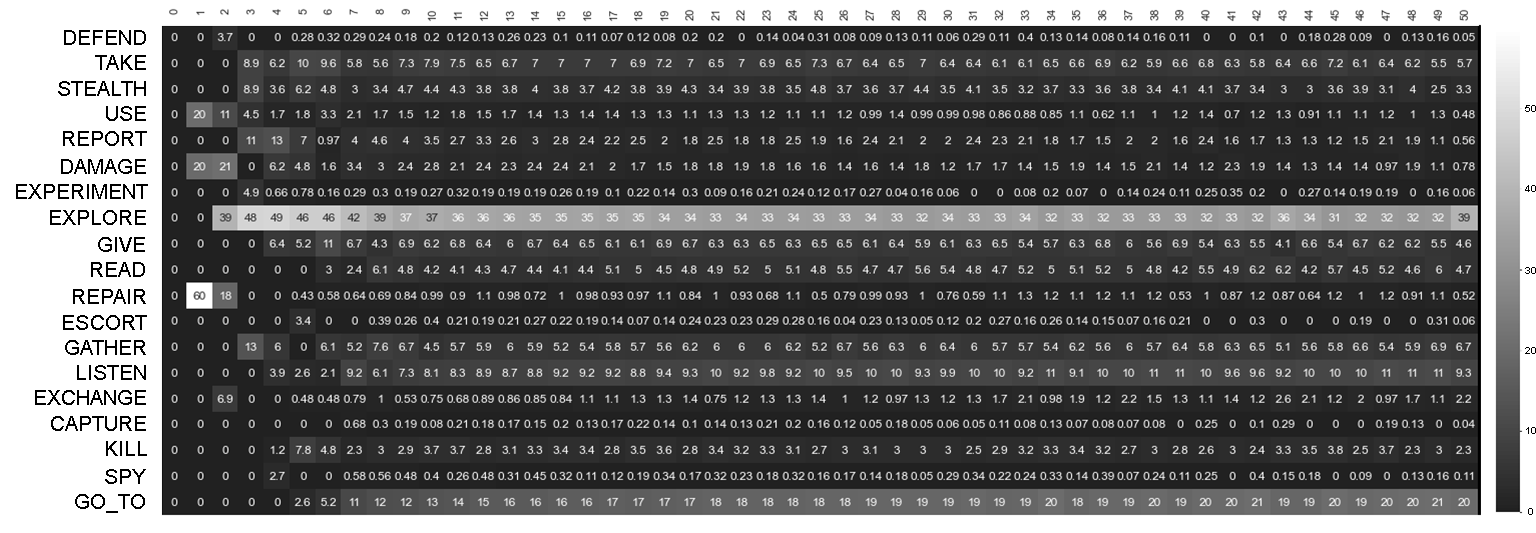
\includegraphics[width=1\textwidth]{included-papers-tex/paper-8/figures/perLengthExperiment-an.png}
        \caption{Chance (in \%) for every quest action (row) to appear in a quest of a given length (column).}
        \label{figs:evaluation:length}
    \end{subfigure} \hfill% \
    %  \captionsetup[subfigure]{width=0.9\textwidth}
    \begin{subfigure}[t]{0.9\textwidth}
        \centering
         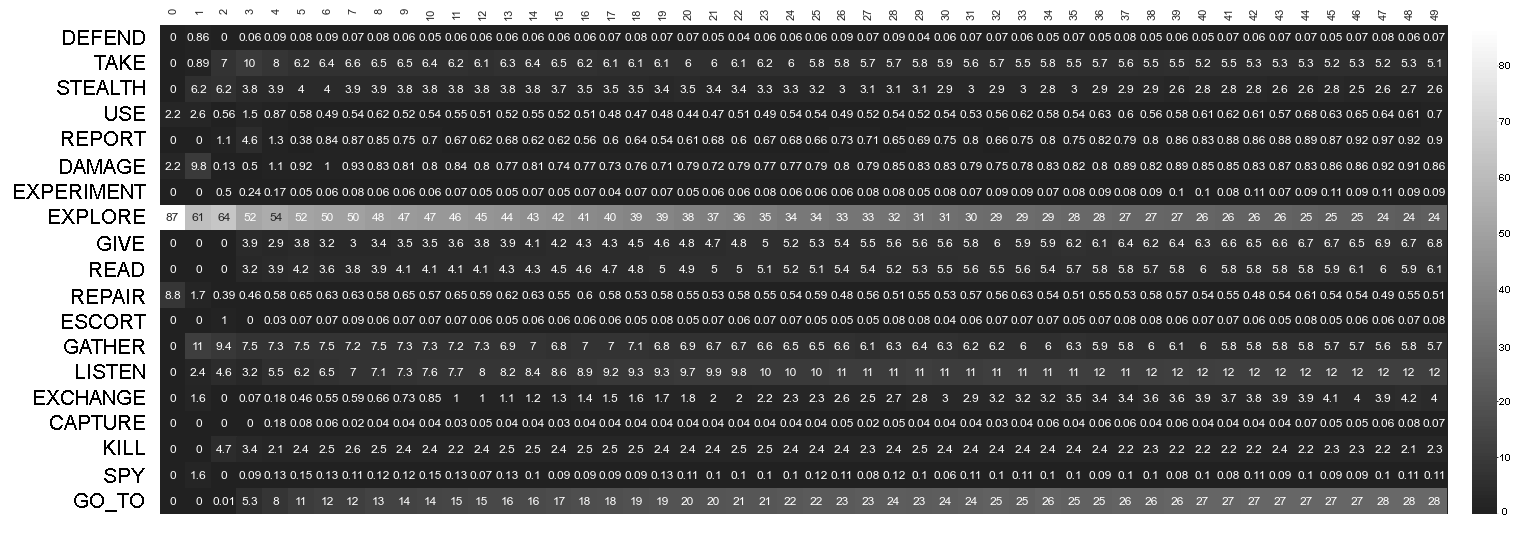
\includegraphics[width=1\textwidth]{included-papers-tex/paper-8/figures/perStepsExperiment-an.png}
        \caption{Chance (in \%) for every action (row) to appear at the Nth step of a quest (column), regardless its length.}
        \label{figs:evaluation:steps}
    \end{subfigure}
    \caption{Results from the Expressive Range Analysis}
    \label{figs:Experiments}
\end{figure*}

\begin{figure}[]
    \centering
    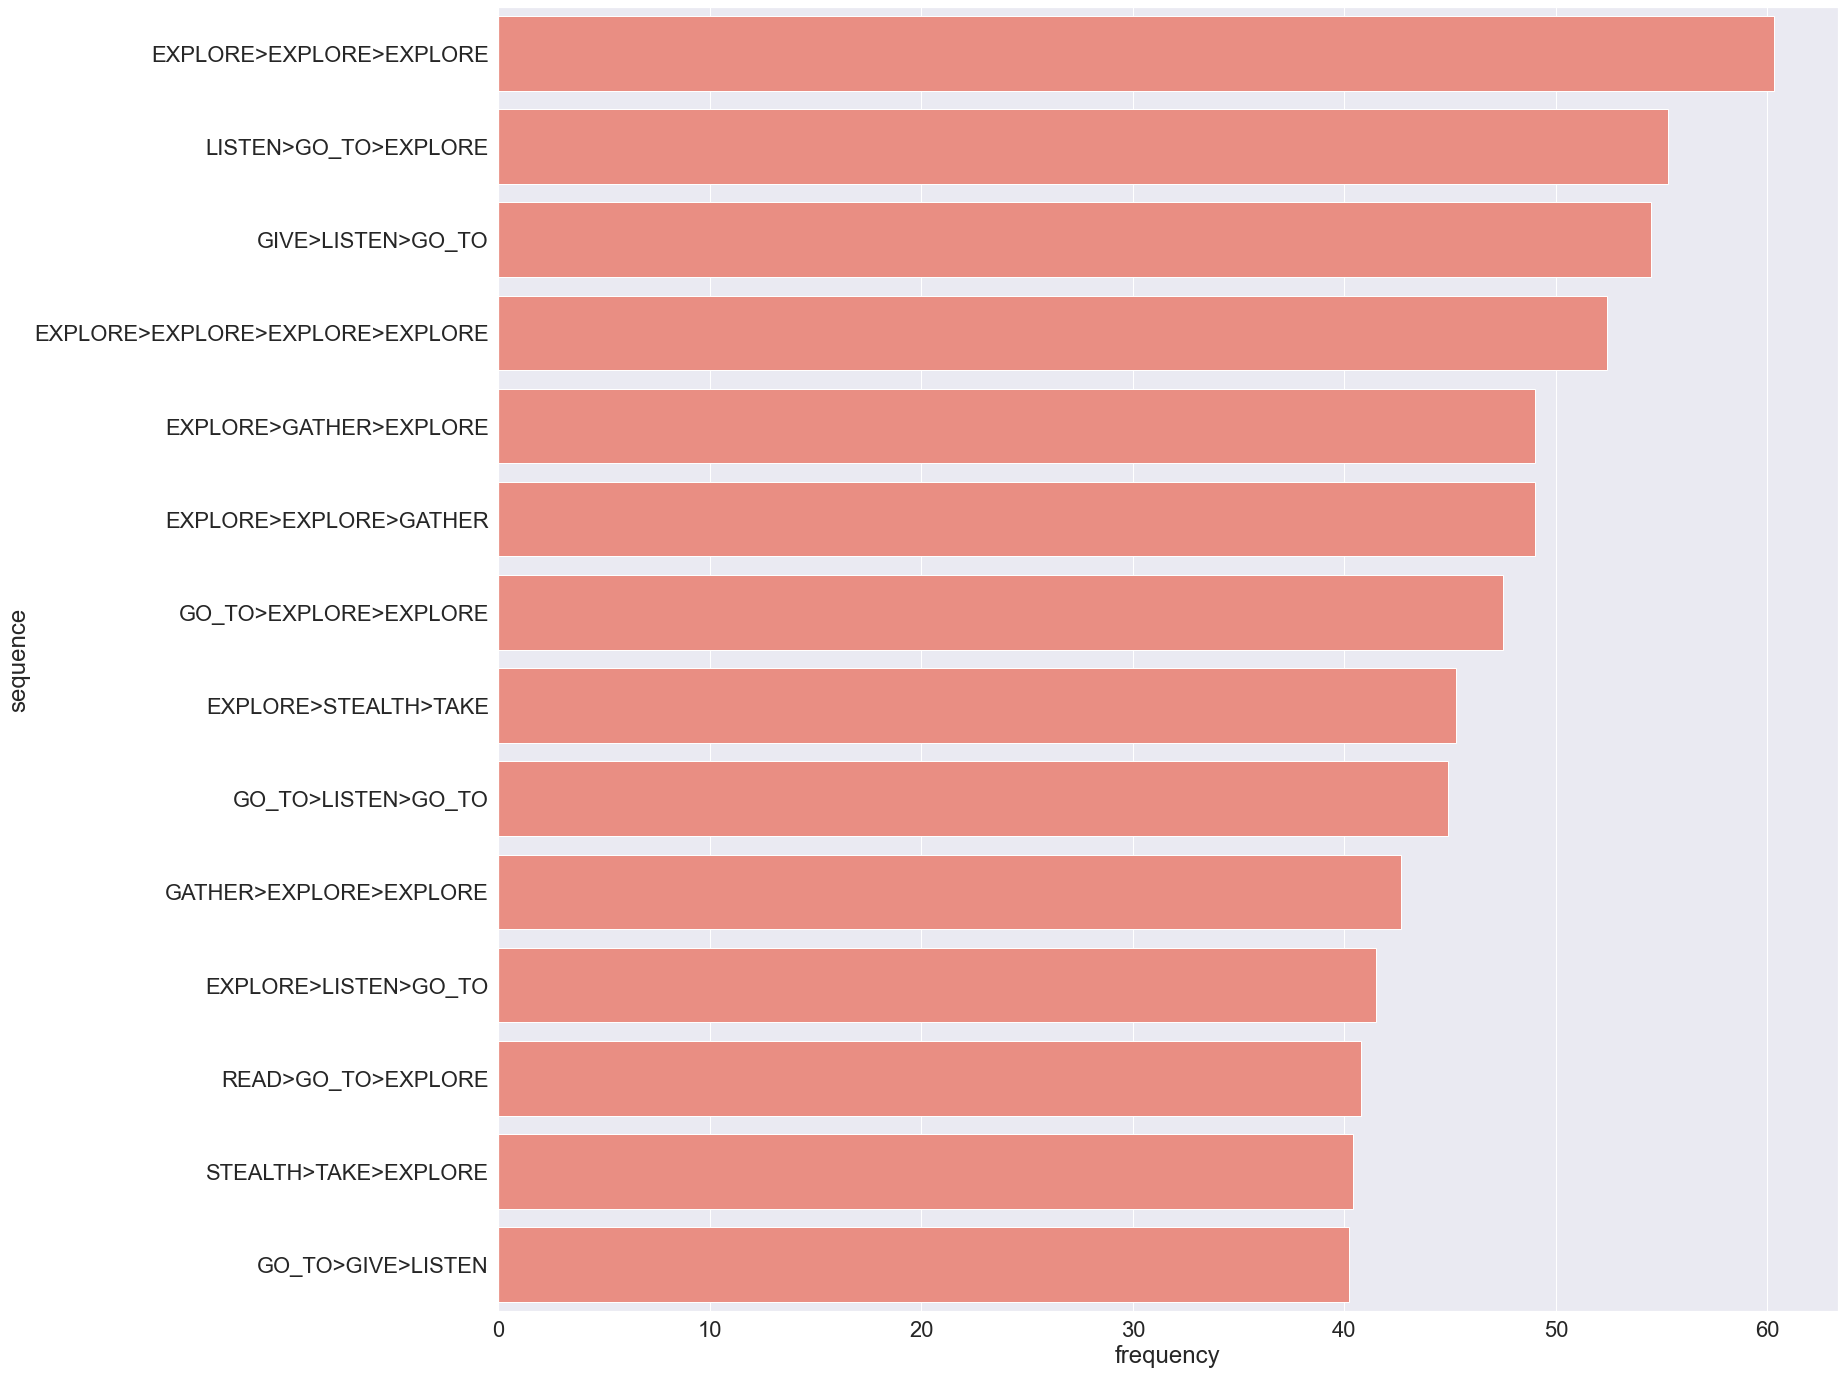
\includegraphics[width=0.9\textwidth]{included-papers-tex/paper-8/figures/CommonSubsequence-GSP.png}
    \caption{Most commonly generated subsequences, with a minimum size of 3.}
    \label{figs:evaluation:CommonSequence}
\end{figure}



\subsubsection{User Study}



% The evaluation of the artefacts usability and functionality was evaluated through a small user study. When evaluating PCG systems, Shaker et. al argues that when making a PCG system, “we are also creating a large amount of content for players to experience, thus it is important to be able to evaluate how successful the generator is according to players who interact with the content”~\citepeighth{p8shaker_procedural_2016}. In our case, EDD is a development tool for designers and not for actual players, but we argue that the actor interacting with the system, in our case, the designer, still is the interactive actor and thus we have decided to do an evaluation with actual potential users of the artefact. An additional advantage of conducting a user study is that it evaluates the aspects that cannot be objectively measured, such as aesthetics and playing experience~\citepeighth{p8Yannakakis2018}. In addition, previous studies on mixed-initiative systems have been conducted through a user study, such as the first version of  EDD[35], its second follow-up study [36] and Sentient Sketchbook [24]. 

% \subsubsection{Results}

Six participants tested our tool following three pre-designed tasks and questionnaires to evaluate Questgram's usability, functionality, and usability. They were all given a document describing the study's purpose and aim, a brief introduction to EDD, and the interview overview. The users were then asked to complete three tasks that covered the tool's functionality and different approaches to creating quests. The tasks were to 1) manually create a quest, 2) automatically create a quest, and 3) create a quest through mixed-initiative. They were also asked to create a dungeon that suited their preferences and objectives before creating quests. The questionnaire consisted of 17 closed-ended questions, and the rest were open-ended. The interview began with a questionnaire with six questions about the users' background and experience within game development and finish with questions about their experience and opinions on the tool. Both the questionnaire and interview followed guidelines described by Oates~\citepeighth{p833-ResearchingInfoSystems}.  

The participants were selected through convenience sampling and were game developers working in game and level design (2) and game development alumni (4), without any experience with EDD or mixed-initiative tools. Five out of six have played dungeon/adventure games and have developed some game with quests and missions, while only two out of six have developed dungeon style games.

\paragraph{Manual Quest Creation}

Participants reported that the tool was easy to use, clear, intuitive, and while simple and basic, it had enough building blocks for them to create their objective quest. Positive feedback was also given regarding the UI, integration with the rest of EDD functionalities, clarity of the quest action concerning the quest, and making the tool overall more interesting. However, some participants expressed confusion when quest sequences became too large as they would have preferred to separate the quests into sections or subquests. Another concern expressed was the inability to change the order of already created quests without redoing the whole quest sequence.

\paragraph{Automatic Quest Creation}

Some participants reported that the system showed potential and a good addition to the manual creation, especially for the creation of side quests such as how similar systems work in \emph{Skyrim}, and for learning how to use the tool as some kind of tutorial. Nevertheless, most participants remarked the system as random and illogical regarding random tile picks connected with quest actions as the system picked farther away NPC and targets with no purpose. In addition, participants felt that a system like this complicated the creation and took the freedom of creating their world and ideas. 

\paragraph{Mixed-Initiative Quest Creation}

The participants described the system as helpful and useful; pointing out that the main advantages and potentials were related to when they reached an inspiration blockage as the designer could get inspired by the suggestions; to allow designers to focus on key parts of a quest sequence, and the speed gained to create quests "in just a matter of moments." While most feedback was positive, there were still concerns among participants regarding the system's cohesiveness as it could feel hard to make the suggestions cohesive with what the participant had in mind. Nevertheless, a majority of the participants experienced that both the manual and automatic complemented each other.

\paragraph{Automatic Suggestions}

Participants generally described the automatic suggestions as useful to gain inspiration, keep the quest creation diverse, and learn what could be created, rather than useful to replace or add to their work. For instance, one participant said that "[the system] suggested to capture a monster which had thought about killing. The "capture" option might be more interesting and might have been an option I had otherwise overlooked." Similarly, another participant pointed out that the automatic suggestions "... were useful in getting inspiration for quests, and to learn the program and what kinds of quests I was actually able to make." Usually, designers have a predetermined idea on how they would like the narrative to unfold. However, based on the responses we received, the system gave a different perspective to the users on what they could create or how they could continue a quest, which makes the tool useful for brainstorming quest design similar to tools such as Questbrowser~\citepeighth{p8Sullivan2009-questbrowser}, albeit constrained to the possible quest actions.

Still, participants preferred to use the system as inspiration rather than effectively incorporating changes to the quests. This was mainly due to the suggestion not feeling cohesive enough with what participants created until then, and the random tiles picked for the quest action. For instance, receiving a "GO TO" suggestion to a random tile on the opposite side of the level and not near the player or the previous quest action.


% However, most participants described the automatic suggestions as inspiring rather than useful to replace or add to their work. 
% It worked well for looking though the options and deciding which would be best to use or to find possibilities that I had not previously considered. They were not very good at applying directly. Say that it suggested to capture a monster which had thought about killing. The "capture" option might be more interesting and might have been an option I had otherwise overlooked. Still not great for suggestions to apply directly but a good way to look at your options.

% This would have good potential for making the designers be able to focus better on the parts that were important in a quest, and let the computer make up the steps inbetween. I think generally it would make a bit more sense for a player to set a start and a goal for a level, then have the computer generate bits in between those.

% The mixed creation was helpfull for me since i like to do it all myself but when i reaced a inspirationblock the automatic came in and helped move it along. The automatic suggestions changed dynamicly with whatever i added to my own questline.

% I liked the possibility to use a suggestion when I wanted inspiration or ran out of ideas myself. For me personally I don't think it's a more efficient way to create quests for the same reason that he suggestions often don't work with the quests that has already been chosen- or that it's just faster to do it manually. So the final thought is that I think that it's a nice thing to have, but I would probably use manual creation more.

% Yes, it was useful. It gives you some ideas to what you can do. You can build further on those ideas. Though it could have been a bit more.

% The automatic suggestions, for me personally, were useful in getting inspiration for quests, and to learn the program and what kinds of quests I was actually able to make. I personally didn't find it useful in speeding up or making the creation more efficient, but it feels like a nice tool to have if you get stuck or want some new ideas.

\paragraph{Quest Actions}

Quest actions and their goals were perceived as easy to understand and suitable for the type of game they were creating, except for "experiment," "stealth," and "spy," since they felt ambiguous and not clear for some participants. Fulfilling some quest actions' prerequisites was somewhat obscure, and some participants needed to go through trial and error to gain access to the quest action. However, once they fulfilled the prerequisites, it was clear and made sense in the context.

\paragraph{Usability}

All participants described the tool as a useful addition for game developers when developing dungeon games but with different arguments and situations on when it would be useful. For instance, to create mundane quests in games with a grinding flow such as \emph{Diablo}, to fast-prototype ideas and systems to give insights into what it might be possible and what might work, and to complement the creation of content and quest-design. Some participants expressed that making the game playable is a must to get the full benefit from the tool.

\paragraph{Creativity}

Most of the participants reported that they experienced increased creativity when using mixed-initiative creation. The participants described that it helped when they got stuck, and it showed different alternatives and routes they did not previously consider. Further, one participant explained that they could make more creative decisions and not "staying safe" and adding "extra steps" without any effort. For instance, using a spy before a kill, thus prolonging the sequence by an extra action. Two participants highlighted that while they did not experience increased creativity, they saw the tool as useful when no new ideas are there given the possible "out of the box" suggestions.

\paragraph{Overall Experience and Missing Features}

Some participants expressed that the tool was useful for someone in the gaming community, but it would be hard to grasp for someone unfamiliar with the concept. Further responses were that it was simple to work with, felt scalable, and the software's recommendation felt useful when designing a quest. Additional response from one participant, who, despite having no prior experience in either creating or playing dungeon games, said it was a fun introduction to the genre and that it was easy to learn and understand. Further, they explained that the simple workflow inspired them to continue creating. In addition, further responses were that the software was quick, feature-rich, simple to use, and got their creativity flowing.

In general, the participants expressed that more interaction with the quest sequence itself, such as changing the order of subsequences, adding quest actions in arbitrary parts, having separate quests, or knowing which quests were manually and automatically, would improve the system considerably. 

\subsubsection{User Study Discussion}

Since we use the work by Doran and Parberry~\citepeighth{p8Doran2011-questsMMORPGs} as a base for the quest generation, this research indirectly tests their quest patterns and their applicability into a mixed-initiative tool. We leveraged on these quest patterns similar as others have on quest patterns~\citepeighth{p8Trenton2010-questpatterns,p8Smith2011-situatingQuests}, and how EDD leverages on level design patterns for the level generation~\citepeighth{p8Baldwin2017,p8alvarez2019empowering}. The use of quest patterns greatly improves the communication with the designers as they can use concepts they feel comfortable with and relate better to the content they create. All of our participants confirmed the previous statement by pointing out how the tool was straightforward, easy to understand with quests actions to be found in any other game type, and easy to use even if they had never used a mixed-initiative tool.
% We leveraged on the quest patterns defined by Doran and Parberry~\citepeighth{p8Doran2011-questsMMORPGs} similarly to how EDD leverages on level design patterns for the level generation facet~\citepeighth{p8Baldwin2017,alvarez2019empowering}.

% Leveraging on game design patterns is not new~\citepeighth{p8Bjork2004-GameDesignPatterns} and similar conclusions have been presented before~\citepeighth{p814-Dahlskog2015-patternsDungeonsGens,Smith2011-situatingQuests,Trenton2010-questpatterns,Baldwin2017,Alvarez2018}; thus, our user study confirms.

Furthermore, while relevant, the suggestions by the system felt impractical mainly and according to participants because the system randomly assigned tiles for the suggested quest action, which limited the tool's perceived usability. Another reason is the use of abstract quest actions. On the one hand, this allows us to disconnect the system from specific implementations and gameplay functionalities of the quests, creating and representing a more generic system. On the other hand, this resulted in a lack of thematic and concrete elements such as NPC roles or defined plot lines and plot elements to follow. These make it harder for designers to contextualize their creations and why the system recommends specific quest actions. %Some preliminary study was done 

%On the other hand, this lack of thematic and concrete elements such as NPC roles, and defined plot lines and elements to follow, makes it harder for designers to contextualize their creations and what or why the system recommends certain quest actions.

Nevertheless, the system was helpful for creativity support and design aid as the suggestions were used as an inspiration to what was possible and what to do next rather than using the actual suggestion. Participants only applied suggestions when the next step felt mundane, and the system suggested a logical position. Leveraging on the human designer for deciding location, while the system provides the quest actions that would follow a more typical quest based on the quest patterns would probably compose a better collaboration. 

%Likewise, this also shows the need for exploring other fundamental and useful ways to establish human-AI collaboration, specifically MI-CC tools that effectively enables the proactive collaboration and creation. Some preliminary study showed that when adding NPC roles and adapting Questgram to it, helps the users contextualize and create quests more alike common quests in RPG. Yet, users used even less the suggested actions as it was seem as "help for novices," rather than a way to create quests between both. This points towards the need to explore other fundamental and more useful ways to establish MI-CC workflows where systems can adapt and create ~\citepeighth{p8Zhu2018-XAIDesignersMICC}. , but reducing even more the use of the suggested actions, 

%Furthermore, while relevant, the suggestions by the system felt impractical because the system randomly assigned tiles for the suggested quest action. This limited the tool's perceived usability as participants used the suggestions more as an inspiration to what was possible and what to do next rather than using the actual suggestion. Participants only used suggestions when the next step felt mundane, and the system suggested a logical position. Leveraging on the human designer for deciding location, while the system provides the quest actions that would follow a more typical quest based on the quest patterns would compose a better collaboration.

%Nevertheless, it is important to point out that we are using and suggesting abstract actions represented in a generic way to disconnect the system from specific implementations. On the one hand, this allows us to to disconnect the system from specific implementations and gameplay functionalities of the quests. On the other hand, this lack of thematic and concrete elements such as NPC roles, defined plot lines 

%While our tool is helpful for creativity support

Some feature suggestions such as separating quests or reordering the quest sequence would have improved the user experience considerably, as after manually placing just a few quest actions, the quest became harder to approach. Even if the system was tested to generate 50 quest actions as explained in section~\nameref{sec:quantExp}, this might be impractical for human designers. An interesting suggestion was to use color tags or similar to understand which agent (Human or machine) created the quest. Then, designers could also use this as a way to understand decisions made by the system and for the system to create a model of the current designer's quests. This could also be used for a collaborative tool where several designers interact with each other and a centralized system; for a more crowdsourced approach such as the one proposed by Charity et al.~\citepeighth{p8charity2020baba}.

%\subsubsection{General Discussion}



%My takeaway from the paper is that support at the level of abstract actions does not provide enough designer support. Designers rarely make use of the suggested actions, but instead use them for inspiration. Further, human designers generally didn’t like the fully automatically generated quests, but instead found them random and illogical. This is ascribed to the random floor tile placement, but I wonder, even with smarter floor tile placement, if the generated quests would still feel unmotivated due to the lack of thematic elements. I would like to hear a discussion from the authors about their conclusions regarding the limits of abstract action grammars, on their own, as design aids. 

%In quests generated by this system, the player spends most of their time just moving around between locations. How can one make all this movement feel motivated for both players and designers? It seems to me that this requires thematic and plot elements. 

%-	In summary, the conclusion I’m drawing from all this as a reader is the somewhat negative result that a grammar of abstract quest actions, on their own, does not provide sufficient quest design support, because of the lack of integration with gameplay, thematic and story elements.  

%R2’s idea is based on the notion that because “[d]esigners rarely make use of the suggested actions,” and found the “fully automatically generated quests… random and illogical,” one way of interpreting these results is as “the somewhat negative result.” That is “a grammar of abstract quest actions, on their own, does not provide sufficient quest design (R2).” From my reading of R2’s review, they are drawing on the often noticed but swept-under-the-rug finding that mixed-initiative tools are most helpful as inspirational aides. But I wanted to point out to the authors that they have a chance here to inspire future creators of mixed-initiative tools by speculating on the limitations of a “grammar of abstract quest actions on their own.” Regardless it would be an interesting avenue for future work/studies.

%-	Another question I had was how the quest actions are supported in the gameplay code. For example, to me the spy action involves watching an NPC to learn some information, while not being observed by the NPC. So, from a gameplay perspective, I could imagine an implementation where the player has to stay outside of the view cone of an NPC, while the NPC performs actions that result in the player learning something. But from the prerequisite table, it sounds like all that is needed is an NPC that the player can move to . 

%Do a bit more discussion on problems with abstract quest design and those things. and the benefits of using these quest design 

% Some feature suggestions, while straightforward such as separating quests or reordering the quest sequence were not implemented 



% \begin{enumerate}
%     \item Manually creating a quest sequence
%     \item Automatically generating a quest sequence
% \end{enumerate}
% \subsection{Concepts and Definitions}

%This paper presents an approach and fundamental steps towards the implementation of designer personas: an analysis of designer style clustering to isolate archetypical paths that can be later be used to build ML surrogate models of archetypal designers. Such models would adapt to the dynamic designer during the mixed-initiative creative process by being placed in the solution space, allowing the designer to traverse such space of models as she drifts through the many dimensions of her creative process.

% design archetypes 

Our work draws from ideas, concepts, and definitions introduced by Liapis et al., such as the core designer model loop when using CAD tools, what can be modeled: preferences, style, goals, processes, and their definition, and particularly, the use of designer modeling as an individual or collective model~\citeptenth{p10Liapis2013-designerModel}. We support our approach on the idea of style as a particular type of designer's preference, and that a collective model can be used to form a stable and static design space, which after being interacted with by designers, can be adapted towards them.

% and the idea of style as a particular type of designer's preference.

%. Moreover, Liapis et al. discuss the modeling of style as a type of preference, where each individual designer has peculiarities and characteristics that makes their style recognizable. While we agree with this vision, we 

%Our work draws from many of the ideas and concepts introduced by Liapis et al.~\citeptenth{p10Liapis2013-designerModel}, in relation to style, goals, preferences and design processes of designers. Nevertheless, given the interdisciplinary scope of this system, and the multiple concepts discussed throughout the paper, it is essential to have operational definitions on the different terms used.

%Thus, in this paper, the shared goal is set and defined by the designer with her design, and as she develops, adapts, and changes, the system seeks to adjust its goals to support the designer's work. Furthermore, the aim of this paper is to propose a system that is able to identify the designer's current goal and style to adapt further the system's goals to provide a personalized experience.

\subsubsection{Design Style} \label{sec:designStyle}

%Every designer has a different style when creating content, especially levels, where one might 

% One idea is to train a supervised learning model on traces of other collaborative creation session and try to predict the next step the human would take in the design process. The main problem with this is that people are different, and different creators will want to take different design actions in the same state;

% One way of overcoming this problem could be to change the level of abstraction at which design actions are modeled and predicted. Instead of predicting individual edits, one could identify different styles or phases of the artifact being created, and model how a designer moves from one to another. To put this concretely in the context of designing rooms for a Zelda-like dungeon crawler~\citeptenth{p10tloz}, one could classify room styles depending on whether they were enemy onslaughts, complex wall mazes, treasure puzzles, and so on. One could then train models to recognize which types of rooms a user creates in which order. By clustering sequences of styles or phases we could formulate designer personas as archetypical trajectories through style space, rather than as sequences of individual edits. For example, in the context of creating a dungeon crawler, some designers might start with the outer walls of the rooms and then populate it with NPCs, whereas another type of designer might first sketch the path they would like the player to take from the entrance to the exit and then add parts of the room outside the main path.

There exist many different styles when creating content, especially levels, that designers can create and adapt to accomplish their goals and the experiences they want for players. On a general level, \emph{Design Style} encompasses the creative process from conceptualization, prototyping, reflection, adaptation, especially when following different processes or constraints during collaboration. Taking a more concrete and operational level, \emph{Design Style} can be analyzed as overarching goals that different designers have when creating a dungeon. For instance, dungeons in games such as Zelda\citeptenth{p10tloz} or The Binding of Isaac\citeptenth{p10mcmillen_binding_2011}, represent a particular playing style planned by the designer. In the former, low tempo, exploring the dungeon, and secret rooms define the style of the dungeons, whereas in the latter, high tempo, optimizing time and resources, small rooms, and in general high-challenge define the dungeons. 

While interesting and relevant to understanding the designers' holistic design process and the expected player experience, \emph{Design Style} can also be discussed on an individual room basis. Rooms have their own set of characteristics and styles that can be identified and modeled to understand their design process. Some would prefer to create the room's architecture first to then create the goals within, whereas others would like to place strategic objectives around and then create the architecture around it or alternating between both. Even with such a division, how to reach those design styles is not straightforward and does not require the same strategy, which also shows the preference and style of individual designers. For instance, if the goal is to create a challenge to reach a door, the designer could create a room with a substantial number of enemies, create a concentrated high-challenge in the center of the room, or divide the room into smaller choke areas. Therefore, in this paper, we take a simplified view of \emph{Design Style} and treat it as the style designers follow to create a room, informed by the individual steps each has taken connected to their preferences and goals.

% While this is a simplified view of \emph{Design Style}, we acknowledge that this is a simplified view of \emph{Design Style}, as this could encompass 

% I take some issue with the framing of the paper as being one of modeling someone’s “design style” based only on the sequence of design actions taken as evidenced in snapshots of a design process. To be clear, I think the snapshot approach is a perfectly reasonable one.  But I worry that giving it a term as all-encompassing as “design style” is overpromising, because there is so much about someone’s approach to design that is lost in reducing it to a sequence of partial designs: moments of self-reflection, prototyping and throwing away ideas before moving to new ones, experimentation on paper away from the machine, prior exposure to design and how it informs new design choices, adherence to norms of genre. Obviously these cannot be captured through this approach, nor do they need to be for the work to be valid. Nonetheless, it seems unfair to characterize “design style” as a mere sequence of edit operations.

% I think more precise language would also make clearer what the strengths and limitations of this study are. By naming the aspects of design that are not captured, it makes clear what potential future work there is, how this approach should and should not be applied in other design tools, and the extent to which this work may be generalizable across tools and genres.

% I think this issue also comes up in cluster labeling. Some of the cluster labels refer to properties of room layout (e.g. “maze-like complex architecture”; “dense room”), some to meta-aspects of design (e.g. “high challenge, clear goal”), some to types of actions (e.g. “separating and populating chambers”, “balancing and optimizing”). It seems like it should be possible for a room to fall into two of these labeled clusters simultaneously (e.g. a maze-like room that has many enemies and a clear goal at the end of the maze), and it’s confusing that these are separate clusters. The same is true for other cluster pairs (e.g. “bordered rooms with deeper architectural development” and “dense, full-range leniency” seem like they could co-exist). It’s also not clear how these cluster labels are applied (other than a “qualitative analysis” — but was this done by the research team, or by external experts? how was this evaluated?).


% we use a simplified vision of \emph{Design Style}

% this general level is interesting to udnerstand the designer's holistic design process, there is a need to 

% analyzing the individual rooms gives a

% Every designer has a different style when creating content, especially levels, some would prefer to create the architecture of the room first to them proceed to create the goals within, whereas others would like to place strategic objectives around and then create the architecture around it or alternating between both. Even with such a division, how to reach those design styles is not straightforward and does not require the same strategy, which also shows the preference and style of individual designers. For instance, if the goal is to create challenge to reach a door, the designer could create a room with a substantial amount of enemies, or create a concentrated high-challenge in the center of the room, or divide the room into smaller choke areas.

% Going to a more general level, one could also think of the designs as overarching goals that different designers have when creating the dungeon. For instance, dungeons in games such as Zelda\citeptenth{p10tloz} or The Binding of Isaac\citeptenth{p10mcmillen_binding_2011}, represents a certain playing style planned by the designer. In the former, low tempo, exploring the dungeon, and secret rooms defines the style of the dungeons, whereas in the latter, high tempo, optimizing time and resources, small rooms, and in general high-challenge. While this general level is interesting to udnerstand the designer's holistic design process, there is a need to 

% the whole dungeon represents a certain playing style the design

% One can also think on the designs as a overaching goals that different designers would have, some would luike a high-tempo with smaller rooms and high challenge with minimal rewards while others might prefer the designer to go through more convoluted mazes with many connections to confuse the player and reward the understanding of patterns. While this view is interesting to understand the designer's holistic design process; in this paper we threat Design Style specifically as the style designers follow to create a room, informed by the individual steps each has taken.


% % I think i should discuss 

% % While very discussed, style 

% We can discuss this in both a specific and general level. For adventure and rogue-like games such as Zelda\citeptenth{p10tloz} or The Binding of Isaac\citeptenth{p10mcmillen_binding_2011}, the whole dungeon represents a certain playing style the design  %in-development

% \subsubsection{Designer's Goals}

% Usually, designers' goals are linked to the experiences they want to create for players, however, in a MI-CC tool, the goal is defined as the 

% It is identified as the 
% The designer's goal is defined as the current state of rooms and the set of interactions done in the tool or sequence of steps taken thus far, to reach such a state. Goals by the designer are linked to the addition and strategic placement of enemies and treasures, giving some goal for the player, e.g., forcing the fight with an enemy or allowing the player to avoid the conflict through side paths.



%Specifically, this definition is used as the current goal to be achieve by the designer identified as the sequence of steps taken thus far. Goals by the designer are linked to the addition and strategic placement of enemies and treasures, which gives some type of goal for the player, e.g. force the fight with an enemy or give the opportunity for the player to avoid the conflict through side paths. 

%Moreover, in EDD the designer is tasked to create a dungeon with an unlimited amount of interconnected rooms where each room can be further designed on it's own. When designing the dungeon and the rooms, the designers have the freedom to create the rooms as they want with any goal for the player. For instance, if the goal of the designer is to create a boss room, she might create a room with some narrow corridors that end up in a fight with a boss.



% \subsubsection{System Goals}

% The system goals are defined as the system's approach to support and foster the work of the designer by providing suggestions aligned with her current design or giving assistance, information, visualization, and measurements when needed. In general, when providing suggestions, the system aims at generating rooms among multiple areas of the generative space, simultaneously providing rooms adapted to the designer's goal and different from it. 




%The system's goal is to support the work of the designer by providing assistance, information, and measurement when needed. The system's main feature is the provided suggestions by means of the Interactive Constrained MAP-Elites~\citeptenth{p10Alvarez2020-ICMAPE}. These suggestions adapts to the current room's design by automatically modifying the fitness function in favor of the new features of the room such as enemy and treasure ratios or the balance between corridors and open chambers. Through this suggestions, the goal is to provide possible designs in the generative space for the designer while fostering her creativity by presenting suggestions that might not have been considered by her.




% \subsubsection{Shared Goals}

% The shared goals between the system and the designer are defined as the goals the designer has when creating the dungeon and the individual rooms. Thus, in this paper, the shared goal is set and defined by the designer with her design, and as she develops, adapts, and changes, the system seeks to adjust its goals to support the designer's work. Furthermore, the aim of this paper is to propose a system that is able to identify the designer's current goal and style to adapt further the system's goals to provide a personalized experience.




% \subsubsection{Design Archetypes}
%   %in-development
% Design archetypes or archetypical designer paths are used to describe and represent design processes' paths taken by designers when creating levels 
% This is akin to player archetypes~\citeptenth{p10bartle1996-taxonomy} that partition players into descriptive categories by analyzing their in-game behavior and reactions, design archetypes or archetypical designer paths are used to describe and represent 

% analyzes the behavior of players  partition players into descriptive categories 
\subsection{Conclusions and Future Work}

This paper presents Questgram [Qg], a quest generation tool with a mixed-initiative approach integrated into the Evolutionary Dungeon Designer. Questgram lets a human designer co-create an overarching quest that fits in a dungeon level, as the dungeon is being developed in the designer. Both map and quest are designed in parallel and with the suggestions provided by EDD. Quests make use of Doran and Parberry's quest structure as production rules in a grammar so that all quests are well-formed with respect to the grammar and the level landscape. We show results from a two-fold evaluation, an expressive range analysis, and a user study. 

The expressive range analysis shows several dominant quest actions and structures, though all types of actions could be generated at a wide range of quest lengths. The mixed-initiative approach was positively met by the user study participants, along with the manual creation. However, automatic creation and automatic suggestions received a mixed response, mainly because of a random placement of position on the actions and the use of abstract quest actions. The tool's overall response was positive, and a majority of the participants reported increased creativity while using the tool. Many participants expressed its usability to gain inspiration, as a solution to inspiration blockages, and as a resource-efficient tool for game developers to use. None of the testers noticed the dominance of some actions detected in the expressive range analysis.

This inspirational use points towards the need to explore other fundamental and more useful ways to establish effective MI-CC workflows where systems can adapt and be effectively employed and used. For instance, some interesting future paths would be to explore the creation of more adaptive collaboration that considers the designer's style or to give more autonomy to the AI to have more participation in the creative process and its effects. Within this, one interesting area is the one of eXplainable AI for Designers~\citepeighth{p8Zhu2018-XAIDesignersMICC} where the goal is to achieve system explainability to improve the collaboration and interaction between human and AIs.

 %how to give more autonomy to the AI system and increasing the trustworthiness on the system how to give more autonomy to the AI system 
%improving MI-CC systems


%For instance, Zhu et al.~\citepeighth{p8Zhu2018-XAIDesignersMICC} proposes 


%For instance, different initiative levels where the AI has more participation, varying autonomy where   Zhu et al.~\citepeighth{p8Zhu2018-XAIDesignersMICC}

%used  than MI-CC points towards a 
%Likewise, this also shows the need for exploring other fundamental and useful ways to establish human-AI collaboration, specifically MI-CC tools that effectively enables the proactive collaboration and creation. Some preliminary study showed that when adding NPC roles and adapting Questgram to it, helps the users contextualize and create quests more alike common quests in RPG. Yet, users used even less the suggested actions as it was seem as "help for novices," rather than a way to create quests between both. This points towards the need to explore other fundamental and more useful ways to establish MI-CC workflows where systems can adapt and create ~\citepeighth{p8Zhu2018-XAIDesignersMICC}. , but reducing even more the use of the suggested actions, 


This research sets the first step toward intertwined story and level mixed-initiative generation on EDD, and future work could be to incorporate quest elements as input in the level generation process so that quests and levels reciprocally influence their generative processes~\citepeighth{p8Liapis2019-OrchestratingGames}. Furthermore, adding semantic evaluation on the generated suggestions would allow Questgram to generate interconnected quests that make sense as subsequent parts of an overarching story plot involving game elements, as well as adding a natural-language generation layer to enhance quests with the automatic generation of detailed descriptions and narratives. Another interesting future research would be to create designer models to adapt quest suggestions to the designer's particular style~\citepeighth{p8Liapis2013-designerModel,p8alvarez2020-designerpersonas}. Finally, more extensive user studies will be conducted to analyze further the tool's usability and intuitiveness. 



% Additionally,  Larger user studies would be conducted to analyze the usability and intuitiveness of the tool interface continuously.


% map locations, NPCs, items, and other game elements. Another interesting future line would be to add a natural-language generation layer to enhance quests with the automatic generation of detailed descriptions and narratives.  






\bibliographystylepeighth{ieeetr}
\bibliographypeighth{included-papers-tex/paper-8/references.bib}